\documentclass[11pt]{article}

\usepackage{amsmath}
\usepackage{amssymb}
\usepackage{amsthm}
\usepackage{physics}
\usepackage[margin=1in]{geometry}
\usepackage{enumitem}
\usepackage{tikz}
\usetikzlibrary{arrows.meta,backgrounds}
\usepackage{xr}
\externaldocument[ch4-]{chapter_04_tangent_spaces}

\newcommand{\TpM}{T_p\mathcal M}
\newcommand{\TpsM}{T_p^*\mathcal M}
\newcommand{\TprsM}{T_p^{(r,s)}\mathcal M}
\newcommand{\Cinf}{C^\infty(\mathcal M)}

\title{Chapter 5 --- Fields\\ \large Exercises}
\author{From Differential Geometry to General Relativity --- Study Companion}
\date{}

\begin{document}
\maketitle

\noindent This file is self-contained: everything needed to state and solve
the problems below is introduced inline, in the book's own notation. Problems
are organized by topic, following the logical order in which the chapter
builds up the theory; within each topic: motivation, notation and
definitions, common pitfalls, problems (easy $\to$ hard), then solutions.

% =============================================================================
\section{Vector Fields and the Tangent Bundle}
% =============================================================================

\subsection*{Motivation}

\paragraph{Why fields.}
A tangent vector lives at a single point, but the objects of physics are spread over space: the velocity of a fluid at every point, the four-velocity of a cloud of dust, the direction of a gravitational acceleration. A \emph{vector field} is a choice of one tangent vector at every point of $\mathcal M$. Everything that compares vectors at different points (derivatives, flows, the directions along which a symmetry acts) needs a field, and needs it to vary smoothly.

\paragraph{Why a bundle.}
The tangent spaces $\TpM$ at different points are different vector spaces, and nothing in their definition says that a vector at $p$ is ``close to'' a vector at a nearby point $q$. To say that a choice $p\mapsto V(p)$ varies smoothly we need the collection of \emph{all} tangent spaces to be a smooth manifold itself, so that ``smooth map into the collection'' has a meaning. That manifold is the tangent bundle; a smooth vector field is then a smooth map that returns, at each $p$, a vector sitting over $p$.

\paragraph{The questions.}
How does one recognise a smooth field in a chart (Problem~\ref{prob:smooth-section-iff-smooth-components})? How are the components of one field in two charts related, and what does a rotation field look like in polar coordinates (Problem~\ref{prob:rotation-field})? What can one do with fields algebraically, besides adding them (the last two topics of this chapter)?

\subsection*{Notation and Definitions}

\noindent Throughout, $(\mathcal M,\mathcal O,\mathcal A)$ is a smooth manifold of dimension $d$ (a topological space with topology $\mathcal O$ and a maximal smooth atlas $\mathcal A$), all scalars are real, and $\Cinf$ is the set of smooth functions $f:\mathcal M\to\mathbb R$, meaning that $f\circ\mathcal X^{-1}:\mathbb R^d\to\mathbb R$ is smooth in the ordinary multivariable sense for every chart $(\mathcal U,\mathcal X)\in\mathcal A$. For a chart, $\mathcal X^i:\mathcal U\to\mathbb R$ is its $i$-th coordinate function, and $\partial_i$ is the ordinary partial derivative with respect to the $i$-th argument of a function on $\mathbb R^d$.

\subsubsection*{Recalled from the pointwise theory}
A tangent vector $v_{\gamma,p}\in\TpM$ is the map $f\mapsto v_{\gamma,p}(f):=(f\circ\gamma)'(\lambda_0)$, where $\gamma$ is a smooth curve with $\gamma(\lambda_0)=p$; $\TpM$ is a $d$-dimensional vector space, and two vectors are equal exactly when they return the same number on every function defined near $p$. For a chart $(\mathcal U,\mathcal X)$ and $p\in\mathcal U$, the chart-induced basis of $\TpM$ is $\left(\frac{\partial}{\partial\mathcal X^i}\right)_p(f):=\partial_i[f\circ\mathcal X^{-1}](\mathcal X(p))$, and every $v\in\TpM$ expands as
\begin{equation}
v=\sum_{i=1}^d v(\mathcal X^i)\left(\frac{\partial}{\partial\mathcal X^i}\right)_p,
\tag{5.1}\label{eq:5-vec-expansion}
\end{equation}
where $v(\mathcal X^i)=(\mathcal X^i\circ\gamma)'(\lambda_0)$ is the $i$-th \emph{component} of $v$ in this chart.

\paragraph{Running example.} Let $\mathcal M:=\mathbb R^2$ with the Cartesian chart $\mathcal X(a,b):=(a,b)$ and the polar chart $\mathcal Y(a,b):=(r,\theta)$, where $a=r\cos\theta$, $b=r\sin\theta$, $r>0$, $\theta\in(-\pi,\pi)$. The polar chart is defined only on $\mathcal V:=\mathbb R^2\setminus\{(a,0)\mid a\le0\}$. We evaluate at
\[
p:=(0,2),\qquad\text{i.e.}\quad r=2,\ \theta=\tfrac\pi2,
\]
which lies in both chart domains.

\subsubsection*{Pointwise operations on scalar fields}
For $f,g\in\Cinf$ and $q\in\mathcal M$ define the \emph{sum} and \emph{product} of scalar fields by
\[
(f\oplus_{C^\infty}g)(q):=f(q)+g(q),\qquad (f\odot_{C^\infty}g)(q):=f(q)\cdot g(q).
\]
Both are again smooth (a sum and a product of smooth real functions). The symbols $\oplus_{C^\infty},\odot_{C^\infty}$ are just ``addition'' and ``multiplication'' of functions, with $C^\infty$ recording the set they act on.

\paragraph{Example.} On $\mathbb R^2$ let $f(a,b):=a^2+b$ and $g(a,b):=a$. Then
\begin{align*}
(f\oplus_{C^\infty}g)(a,b)&=a^2+a+b,\\
(f\odot_{C^\infty}g)(a,b)&=a^3+ab,
\end{align*}
and at $q=(1,2)$ the values are $f(q)+g(q)=3+1=4$ and $f(q)\,g(q)=3\cdot1=3$, in agreement with $a^2+a+b=4$ and $a^3+ab=3$.

\subsubsection*{Bundles, fibres and sections}
A triple $(\mathcal E,\mathcal O_{\mathcal E},\mathcal A_{\mathcal E})\xrightarrow{\ \pi\ }(\mathcal B,\mathcal O_{\mathcal B},\mathcal A_{\mathcal B})$ of two smooth manifolds and a smooth surjective map $\pi:\mathcal E\to\mathcal B$ is a \emph{(smooth) bundle}: $\mathcal E$ is the \emph{total space}, $\mathcal B$ the \emph{base space} and $\pi$ the \emph{projection}. The \emph{fibre} over $q\in\mathcal B$ is the set $\mathrm{prim}_\pi(q)\subseteq\mathcal E$ of points that $\pi$ sends to $q$ (``prim'' is short for \emph{preimage}). A \emph{section} is a map $\sigma:\mathcal B\to\mathcal E$ with
\[
\pi\circ\sigma=\mathrm{id}_{\mathcal B},
\]
where $\mathrm{id}_{\mathcal B}(q):=q$ is the identity map of $\mathcal B$; that is, $\sigma$ picks one point in each fibre.

\paragraph{Example.} Let $\mathcal E=\mathbb R^2$, $\mathcal B=\mathbb R$ and $\pi(a,b):=a$. The fibre over $3$ is the vertical line $\{(3,b)\mid b\in\mathbb R\}$. The map $\sigma(a):=(a,a^2)$ is a section, since $\pi(\sigma(a))=a$; the map $\tau(a):=(a+1,0)$ is not, since $\pi(\tau(a))=a+1\neq a$.

\subsubsection*{The tangent bundle}
The \emph{tangent bundle} of $\mathcal M$ is the bundle $T\mathcal M\xrightarrow{\ \pi\ }\mathcal M$ with:
\begin{itemize}
  \item total space $T\mathcal M:=\bigsqcup_{p\in\mathcal M}\TpM$, the disjoint union of all tangent spaces, and projection $\pi(v_{\gamma,p}):=p$, so the fibre over $p$ is $\TpM$;
  \item a topology $\mathcal O_{T\mathcal M}$ for which $\pi$ is continuous (the book takes $\mathcal O_{T\mathcal M}:=\{\mathrm{prim}_\pi(\mathcal U)\mid\mathcal U\in\mathcal O\}$, the coarsest such topology);
  \item for each chart $(\mathcal U,\mathcal X)\in\mathcal A$, a chart $\xi_{\mathcal X}:T\mathcal U\to\mathbb R^{2d}$ on $T\mathcal U:=\mathrm{prim}_\pi(\mathcal U)$, given by
  \[
  \xi_{\mathcal X}(v):=\big(\mathcal X^1(p),\dots,\mathcal X^d(p)\,;\,v(\mathcal X^1),\dots,v(\mathcal X^d)\big),\qquad p:=\pi(v),
  \]
  (base-point coordinates followed by fibre components), which together form the atlas $\mathcal A_{T\mathcal M}$.
\end{itemize}
This makes $T\mathcal M$ a smooth manifold of dimension $2d$: $d$ numbers to locate $p$ and $d$ numbers to specify a vector at $p$.

\paragraph{Example.} Let $\mathcal M=\mathbb R$ with the chart $\mathcal X=\mathrm{id}$ ($d=1$). The curve $\gamma(\lambda):=\lambda^2$ at $\lambda_0=1$ has $p=1$ and $(\mathcal X\circ\gamma)'(1)=2$, so
\[
\xi_{\mathcal X}(v_{\gamma,1})=(1\,;\,2)\in\mathbb R^2.
\]
The different curve $\delta(\lambda):=2\lambda-1$ also passes through $1$ at $\lambda_0=1$ with $\delta'(1)=2$; it has the same image $(1;2)$, consistently with $v_{\delta,1}=v_{\gamma,1}$ (same base point, same velocity). Thus $T\mathbb R$ is covered by one chart with values in $\mathbb R^2$.

\subsubsection*{Vector fields}
A \emph{smooth vector field} is a smooth section of the tangent bundle,
\[
V:\mathcal M\to T\mathcal M,\qquad \pi\circ V=\mathrm{id}_{\mathcal M},
\]
so $V(p)\in\TpM$ for every $p\in\mathcal M$. (Problems below write a generic field as $\mathcal X$; here fields are $V,W$ to keep the letter $\mathcal X$ for the chart.) A field acts on $f\in\Cinf$ by
\[
V[f]:\mathcal M\to\mathbb R,\qquad V[f](p):=V(p)(f),
\]
the derivative of $f$ in the direction $V(p)$ at each point $p$; $V[f]\in\Cinf$ and $f\mapsto V[f]$ is $\mathbb R$-linear. On a chart domain $\mathcal U$ the \emph{component functions} of $V$ are
\[
V^i:=V[\mathcal X^i]:\mathcal U\to\mathbb R,\qquad i=1,\dots,d,
\]
so by \eqref{eq:5-vec-expansion}, for every $p\in\mathcal U$ and $f\in\Cinf$,
\begin{align*}
V(p)&=\sum_{i=1}^dV^i(p)\left(\frac{\partial}{\partial\mathcal X^i}\right)_p,\\
V[f](p)&=\sum_{i=1}^dV^i(p)\,\partial_i[f\circ\mathcal X^{-1}](\mathcal X(p)).
\end{align*}
Applying the bundle chart $\xi_{\mathcal X}$ to $V(p)$ gives
\[
\xi_{\mathcal X}(V(p))=\big(\mathcal X(p)\,;\,V^1(p),\dots,V^d(p)\big),
\]
so $V$ is smooth as a map into $T\mathcal M$ exactly when its component functions are smooth in every chart (Problem~\ref{prob:smooth-section-iff-smooth-components}).

\paragraph{Example: the shear field.} On $\mathbb R^2$ with the Cartesian chart, let $V$ have components
\[
V^1(a,b):=b,\qquad V^2(a,b):=0.
\]
They are polynomials, hence smooth, so $V$ is a smooth vector field: it pushes points to the right above the $a$-axis and to the left below it, and vanishes on the $a$-axis. For $f(a,b):=a^2+b$,
\[
V[f](a,b)=b\,\partial_af+0\cdot\partial_bf=2ab,
\]
and at $p=(1,2)$ the vector is $V(p)=2\left(\frac{\partial}{\partial\mathcal X^1}\right)_p$, so
\[
V(p)(f)=2\cdot\partial_af(p)=2\cdot2=4=V[f](p).
\]

\paragraph{Example: a section that is not smooth.} On $\mathbb R^2$ let $W^1(a,b):=|b|$ and $W^2(a,b):=0$. This defines a vector $W(p)\in\TpM$ at every $p$, i.e.\ a section of $T\mathbb R^2$, even a continuous one. But $|b|$ is not differentiable at $b=0$, so by the criterion above $W$ is not a smooth vector field.

\subsubsection*{Sum and rescaling of vector fields}
Let $\Gamma T\mathcal M$ be the set of smooth vector fields on $\mathcal M$. For $V_1,V_2,V\in\Gamma T\mathcal M$, $f,g\in\Cinf$ and $p\in\mathcal M$ define $V_1\oplus_\Gamma V_2$ and $f\odot_\Gamma V$ through their action on functions,
\begin{align*}
(V_1\oplus_\Gamma V_2)[g](p)&:=\big(V_1[g]\oplus_{C^\infty}V_2[g]\big)(p),\\
(f\odot_\Gamma V)[g](p)&:=\big(f\odot_{C^\infty}V[g]\big)(p),
\end{align*}
where $\Gamma$ (for \emph{sections}) records that these operations act on fields. They are smooth vector fields again (Problem~\ref{prob:module-axioms}). Because a vector is determined by its action on functions, they are the pointwise operations, and in components
\[
(V_1\oplus_\Gamma V_2)^i=V_1^i\oplus_{C^\infty}V_2^i,\qquad (f\odot_\Gamma V)^i=f\odot_{C^\infty}V^i.
\]

\paragraph{Example.} Let $V$ be the shear field, $W':=\partial/\partial\mathcal X^2$ the constant field with components $(0,1)$, and $f(a,b):=a$. Then
\begin{align*}
(V\oplus_\Gamma W')^i&=(b,\,1),\\
(f\odot_\Gamma V)^i&=(ab,\,0),
\end{align*}
and at $q=(1,2)$ the second field has components
\[
(f\odot_\Gamma V)(q)=(2,0)=f(q)\cdot V(q),
\]
the vector $V(q)=(2,0)$ rescaled by the number $f(q)=1$. Using $g(a,b)=a^2+b$ as above, the definition gives
\[
(V\oplus_\Gamma W')[g](a,b)=2ab+\partial_bg=2ab+1,
\]
the sum of $V[g]=2ab$ and $W'[g]=1$.

\subsubsection*{Changing chart}
Let $(\mathcal U,\mathcal X)$ and $(\mathcal V,\mathcal Y)$ be charts and $p\in\mathcal U\cap\mathcal V$. The \emph{Jacobian} of the change of chart has entries
\[
(J_{\mathcal{VU}})^k_i(p):=\left(\frac{\partial\mathcal Y^k}{\partial\mathcal X^i}\right)_p:=\partial_i[\mathcal Y^k\circ\mathcal X^{-1}](\mathcal X(p)),
\]
with $k$ the row and $i$ the column index, and $(J_{\mathcal{UV}})^i_k(p):=\partial_k[\mathcal X^i\circ\mathcal Y^{-1}](\mathcal Y(p))$ is its inverse matrix. Write $V^i$ and $\widetilde V^k$ for the component functions of $V$ in the charts $\mathcal X$ and $\mathcal Y$. Since the vector $V(p)$ does not depend on the chart, its two expansions coincide, which yields the \emph{contravariant law}
\begin{equation}
\widetilde V^k(p)=\sum_{i=1}^d(J_{\mathcal{VU}})^k_i(p)\,V^i(p).
\tag{5.2}\label{eq:5-vec-comp-law}
\end{equation}
This is the pointwise law of the previous chapter applied at every $p$ of the overlap, and its field-level derivation is Problem~\ref{prob:field-level-transformation-derivation}. Both $V^i$ and $\widetilde V^k$ are functions, defined on $\mathcal U$ and $\mathcal V$ respectively, so \eqref{eq:5-vec-comp-law} is an identity of functions on $\mathcal U\cap\mathcal V$.

\paragraph{Example.} For the shear field at $p=(0,2)$, differentiating $r=\sqrt{a^2+b^2}$ and $\theta=\operatorname{atan2}(b,a)$ gives
\[
J_{\mathcal{VU}}(p)=\begin{pmatrix}a/r&b/r\\-b/r^2&a/r^2\end{pmatrix}=\begin{pmatrix}0&1\\-\tfrac12&0\end{pmatrix},\qquad (V^1,V^2)(p)=(2,0),
\]
so \eqref{eq:5-vec-comp-law} gives
\begin{align*}
\widetilde V^1(p)&=0\cdot2+1\cdot0=0,\\
\widetilde V^2(p)&=-\tfrac12\cdot2+0\cdot0=-1.
\end{align*}
The polar components $(0,-1)$ say that at the top of the circle the shear field has no radial part and moves along decreasing $\theta$ (clockwise), as expected for a push towards $+a$ at $(0,2)$. Directly, the Cartesian and polar basis vectors at $p$ are related by $\left(\frac{\partial}{\partial\mathcal X^1}\right)_p=-\tfrac12\left(\frac{\partial}{\partial\mathcal Y^2}\right)_p$, so
\[
V(p)=2\left(\frac{\partial}{\partial\mathcal X^1}\right)_p=-1\cdot\left(\frac{\partial}{\partial\mathcal Y^2}\right)_p,
\]
the same result.

\subsection*{Common pitfalls and limitations}

\begin{itemize}
  \item \textbf{A section is not automatically smooth.} $p\mapsto V(p)\in\TpM$ is an arbitrary choice unless the components are smooth; $W=|b|\,\partial/\partial\mathcal X^1$ above is continuous but not smooth. Smoothness of the components must be checked in (every) chart.
  \item \textbf{Components are chart-dependent, the field is not.} The shear field has components $(2,0)$ at $p$ in the Cartesian chart and $(0,-1)$ in the polar one. A list of component functions means nothing until the chart is named, and two fields are equal only if they agree at every point, not if their lists look alike.
  \item \textbf{Both charts must contain the point.} \eqref{eq:5-vec-comp-law} holds on $\mathcal U\cap\mathcal V$ only: the polar components of the shear field exist only off the non-positive $a$-axis, although the field itself is defined on all of $\mathbb R^2$.
  \item \textbf{$V[f]$ is a function, $V(p)(f)$ is a number.} The first is a scalar field (the directional derivative at every point); the second is its value at $p$, as in $V[f](p)=4$ above.
  \item \textbf{$\dim T\mathcal M=2d$, not $d$.} Only each fibre $\TpM$ has dimension $d$; the extra $d$ coordinates of $T\mathcal M$ locate the base point. A vector field is a section, which uses only $d$ functions of $p$ (its components).
  \item \textbf{Vectors at different points cannot be added.} Adding fields is done pointwise, vector by vector in the same $\TpM$; the rescaling $f\odot_\Gamma V$ uses a \emph{function} $f$, so different points are rescaled by different numbers.
  \item \textbf{Standing assumptions.} Finite dimension $d$, real scalars and a smooth (not merely topological) manifold: without the smooth structure there is no $T\mathcal M$ as defined here.
\end{itemize}

\subsection*{Problems}

\begin{enumerate}[label=\textbf{5.\arabic*}, leftmargin=2.2cm, start=1]

\item \label{prob:radial-field}
Let $\mathcal M=\mathbb R^2$ with Cartesian chart $\mathcal X=\mathrm{id}$,
and define $\mathcal X_{\mathrm{rad}}:\mathcal M\to T\mathcal M$ by its
components $X^1(a,b):=a$, $X^2(a,b):=b$ in this chart (the ``radial''
vector field). Verify that $X^1,X^2\in\Cinf$, and sketch (in words) what
this vector field looks like at a few sample points.

\item \label{prob:smooth-section-iff-smooth-components}
Let $\mathcal X:\mathcal M\to T\mathcal M$ be a section of the tangent
bundle (i.e.\ $\pi\circ\mathcal X=\mathrm{id}_{\mathcal M}$, not
necessarily smooth yet). Show that $\mathcal X$ is a \emph{smooth} vector
field if and only if, for every chart $(\mathcal U,\mathcal X_{\mathrm{ch}})$
in the atlas, the component functions $\dot\gamma^i_{\mathcal
U}(\lambda_0)$ of $\mathcal X(p)$ (as $p$ ranges over $\mathcal U$) are
smooth ($C^\infty$) real-valued functions of $p\in\mathcal U$. [Use that
$\mathcal X$ is smooth as a map $\mathcal M\to T\mathcal M$ exactly when
$\xi_{\mathcal X_{\mathrm{ch}}}\circ\mathcal X\circ\mathcal
X_{\mathrm{ch}}^{-1}:\mathbb R^d\to\mathbb R^{2d}$ is smooth in the usual
multivariable sense, for every chart of the bundle atlas
$\mathcal A_{T\mathcal M}$.]

\item \label{prob:rotation-field}
Let $\mathcal M=\mathbb R^2\setminus\{(0,0)\}$ with the Cartesian chart
$\mathcal X$ and polar chart $\mathcal Y$ of
Problem~\ref{ch4-prob:jacobian-numeric}. Define a vector field $\mathcal
X_{\mathrm{rot}}$ with Cartesian components $X^1(a,b):=-b$, $X^2(a,b):=a$.
\begin{enumerate}[label=(\alph*)]
  \item Show $\mathcal X_{\mathrm{rot}}$ is smooth.
  \item Using the contravariant component transformation law and the
  Jacobians of Problem~\ref{ch4-prob:jacobian-numeric}, compute the polar
  components $Y^1$ (the $r$-component) and $Y^2$ (the $\theta$-component)
  of $\mathcal X_{\mathrm{rot}}$ at $p=(1,1)$, and interpret the result
  physically (this field generates rotations about the origin, the
  differential-geometric analogue of an angular-momentum/Killing-vector
  flow).
\end{enumerate}

\end{enumerate}

\subsection*{Solutions}

\subsubsection*{Solution 5.1}

\noindent\textit{Statement.} Let $\mathcal M=\mathbb R^2$ with Cartesian
chart $\mathcal X=\mathrm{id}$, and define $\mathcal
X_{\mathrm{rad}}:\mathcal M\to T\mathcal M$ by its components
$X^1(a,b):=a$, $X^2(a,b):=b$ in this chart. Verify that
$X^1,X^2\in\Cinf$, and sketch (in words) what this vector field looks like
at a few sample points.

\medskip
\noindent\textit{Solution.} Recall $f\in\Cinf$ means $f:\mathcal
M\to\mathbb R$ is such that $f\circ\mathcal X^{-1}:\mathbb R^2\to\mathbb R$
is smooth in the ordinary multivariable sense. Since $\mathcal
X=\mathrm{id}$, $X^1\circ\mathcal X^{-1}(a,b)=a$ and $X^2\circ\mathcal
X^{-1}(a,b)=b$: these are the two coordinate projections
$\mathbb R^2\to\mathbb R$, which are polynomials (of degree $1$) in
$(a,b)$, hence $C^\infty$. So $X^1,X^2\in\Cinf$.

At a point $p=(a,b)$, the vector $\mathcal X_{\mathrm{rad}}(p)$ has
Cartesian components $(a,b)$, i.e.\ it points from the origin towards $p$
itself, with length $\sqrt{a^2+b^2}$ equal to the distance from $p$ to the
origin. Thus at $(1,0)$ the vector is $(1,0)$ (unit length, pointing along
the positive first axis); at $(0,2)$ it is $(0,2)$ (pointing along the
positive second axis, twice as long); at $(-1,-1)$ it is $(-1,-1)$
(pointing further away from the origin, into the third quadrant); and at
the origin itself the vector is $(0,0)$. Overall, $\mathcal
X_{\mathrm{rad}}$ points radially outward everywhere, growing linearly in
length with distance from the origin.

\subsubsection*{Solution 5.2}

\noindent\textit{Statement.} Let $\mathcal X:\mathcal M\to T\mathcal M$ be
a section of the tangent bundle (i.e.\ $\pi\circ\mathcal
X=\mathrm{id}_{\mathcal M}$, not necessarily smooth yet). Show that
$\mathcal X$ is a smooth vector field if and only if, for every chart
$(\mathcal U,\mathcal X_{\mathrm{ch}})$ in the atlas, the component
functions $\dot\gamma^i_{\mathcal U}(\lambda_0)$ of $\mathcal X(p)$ (as $p$
ranges over $\mathcal U$) are smooth real-valued functions of $p\in
\mathcal U$.

\medskip
\noindent\textit{Solution.} By definition, $\mathcal X$ is smooth
(as a map between the smooth manifolds $\mathcal M$ and $T\mathcal M$)
exactly when, for every chart $(\mathcal U,\mathcal X_{\mathrm{ch}})$ of
the atlas $\mathcal A$ (with induced bundle chart $\xi_{\mathcal
X_{\mathrm{ch}}}$), the map
\[
\xi_{\mathcal X_{\mathrm{ch}}}\circ\mathcal X\circ\mathcal X_{\mathrm{ch}}^{-1}:\mathbb R^d\to\mathbb R^{2d}
\]
is smooth in the usual multivariable sense on its domain
$\mathcal X_{\mathrm{ch}}(\mathcal U)\subseteq\mathbb R^d$.

Fix such a chart and let $a\in\mathcal X_{\mathrm{ch}}(\mathcal U)$, so
$p:=\mathcal X_{\mathrm{ch}}^{-1}(a)\in\mathcal U$. By definition of the
bundle chart $\xi_{\mathcal X_{\mathrm{ch}}}$, $v_{\gamma,p}\mapsto(\dots,
\mathcal X_{\mathrm{ch}}^i(p),\dots\,;\,\dots,\dot\gamma^i_{\mathcal
U}(\lambda_0),\dots)$, applying it to $\mathcal X(p)=v_{\gamma,p}$ gives
\[
\big(\xi_{\mathcal X_{\mathrm{ch}}}\circ\mathcal X\circ\mathcal X_{\mathrm{ch}}^{-1}\big)(a) = \big(\underbrace{a^1,\dots,a^d}_{=\,\mathcal X_{\mathrm{ch}}(p)},\ \underbrace{\dot\gamma^1_{\mathcal U}(\lambda_0),\dots,\dot\gamma^d_{\mathcal U}(\lambda_0)}_{\text{components of }\mathcal X(p)}\big),
\]
where the first block is just $a=\mathcal X_{\mathrm{ch}}(p)$ (since
$p=\mathcal X_{\mathrm{ch}}^{-1}(a)$), and the second block is the tuple of
component functions of $\mathcal X$, evaluated at $p=\mathcal
X_{\mathrm{ch}}^{-1}(a)$, i.e.\ the functions $\dot\gamma^i_{\mathcal
U}(\lambda_0)\circ\mathcal X_{\mathrm{ch}}^{-1}$ of $a$.

The first block, $a\mapsto a$, is the identity map on $\mathbb R^d$ and is
always smooth. Hence $\xi_{\mathcal X_{\mathrm{ch}}}\circ\mathcal
X\circ\mathcal X_{\mathrm{ch}}^{-1}$ is smooth if and only if each of the
$d$ component functions in the second block,
$\dot\gamma^i_{\mathcal U}(\lambda_0)\circ\mathcal X_{\mathrm{ch}}^{-1}$,
is smooth as a map $\mathbb R^d\to\mathbb R$ — which is exactly the
definition of the component function $\dot\gamma^i_{\mathcal
U}(\lambda_0)$ (as a function of $p\in\mathcal U$) being an element of
$\Cinf(\mathcal U)$.

Since this equivalence holds chart by chart, and $\mathcal X$ is smooth
(as a map $\mathcal M\to T\mathcal M$) iff it is smooth in every chart of
the bundle atlas $\mathcal A_{T\mathcal M}$ (equivalently, in the chart
induced by every chart of $\mathcal A$), $\mathcal X$ is a smooth vector
field if and only if the component functions
$\dot\gamma^i_{\mathcal U}(\lambda_0)$ are smooth for every chart
$(\mathcal U,\mathcal X_{\mathrm{ch}})\in\mathcal A$.

\subsubsection*{Solution 5.3}

\noindent\textit{Statement.} Let $\mathcal M=\mathbb R^2\setminus\{(0,0)\}$
with the Cartesian chart $\mathcal X$ and polar chart $\mathcal Y$ of
Problem~\ref{ch4-prob:jacobian-numeric}. Define a vector field $\mathcal
X_{\mathrm{rot}}$ with Cartesian components $X^1(a,b):=-b$,
$X^2(a,b):=a$.
\begin{enumerate}[label=(\alph*)]
  \item Show $\mathcal X_{\mathrm{rot}}$ is smooth.
  \item Using the contravariant component transformation law and the
  Jacobians of Problem~\ref{ch4-prob:jacobian-numeric}, compute the polar
  components $Y^1$ (the $r$-component) and $Y^2$ (the $\theta$-component)
  of $\mathcal X_{\mathrm{rot}}$ at $p=(1,1)$, and interpret the result
  physically.
\end{enumerate}

\medskip
\noindent\textit{Solution.}

(a) As in Solution~5.1, $\mathcal X=\mathrm{id}$, so $X^1\circ\mathcal
X^{-1}(a,b)=-b$ and $X^2\circ\mathcal X^{-1}(a,b)=a$ are polynomials in
$(a,b)$, hence $C^\infty$; by Solution~5.2 (applied to the single
Cartesian chart, plus smoothness of the transition to any other chart of
the atlas, guaranteed by the smooth-manifold structure) this makes
$\mathcal X_{\mathrm{rot}}$ a smooth vector field.

(b) The contravariant transformation law for vector components (derived
earlier in this chapter) reads, for the change from chart $\mathcal X$ to
chart $\mathcal Y$,
\[
Y^i(p) = \sum_{j=1}^2 (J_{\mathcal{YX}})^i_j(p)\,X^j(p),\qquad (J_{\mathcal{YX}})^i_j(p):=\left(\frac{\partial\mathcal Y^i}{\partial\mathcal X^j}\right)_p.
\]
At $p=(1,1)$ (so $a=b=1$, $r=\sqrt2$), with $\mathcal Y^1=r=\sqrt{a^2+b^2}$
and $\mathcal Y^2=\theta=\arctan(b/a)$ (on the branch containing $p$),
\[
\frac{\partial r}{\partial a} = \frac ar,\qquad \frac{\partial r}{\partial b}=\frac br,\qquad \frac{\partial\theta}{\partial a} = \frac{-b}{a^2+b^2},\qquad \frac{\partial\theta}{\partial b}=\frac{a}{a^2+b^2},
\]
so at $p=(1,1)$ (where $a=b=1$, $a^2+b^2=2$, $r=\sqrt2$),
\[
(J_{\mathcal{YX}})^1_1(p)=\frac{1}{\sqrt2},\quad (J_{\mathcal{YX}})^1_2(p)=\frac{1}{\sqrt2},\quad (J_{\mathcal{YX}})^2_1(p)=-\frac12,\quad (J_{\mathcal{YX}})^2_2(p)=\frac12.
\]
With $X^1(p)=-b=-1$, $X^2(p)=a=1$,
\begin{align*}
Y^1(p) &= (J_{\mathcal{YX}})^1_1(p)\,X^1(p)+(J_{\mathcal{YX}})^1_2(p)\,X^2(p) = \frac{1}{\sqrt2}(-1)+\frac{1}{\sqrt2}(1) = 0, \\
Y^2(p) &= (J_{\mathcal{YX}})^2_1(p)\,X^1(p)+(J_{\mathcal{YX}})^2_2(p)\,X^2(p) = -\frac12(-1)+\frac12(1) = 1.
\end{align*}
So the $r$-component vanishes and the $\theta$-component equals $1$: at
$p$, $\mathcal X_{\mathrm{rot}}$ is purely azimuthal, with unit angular
rate $d\theta/d\lambda=1$ and no radial component. Physically this is the
velocity field of rigid rotation about the origin at unit angular
velocity — the flow it generates is $\lambda\mapsto(\cos\lambda\cdot
a-\sin\lambda\cdot b,\ \sin\lambda\cdot a+\cos\lambda\cdot b)$, i.e.\
rotation by angle $\lambda$ — the differential-geometric analogue of an
angular-momentum/Killing-vector flow.

% =============================================================================
\section{Covector Fields and the Cotangent Bundle}
% =============================================================================

\subsection*{Motivation}

\paragraph{Why covector fields.}
A vector field says \emph{where things move}; a covector field says \emph{how a direction is measured}. The work done by a force along a displacement, the change of a potential along a path, the gradient of a temperature: each is a rule that eats a tangent vector at every point and returns a number, linearly. A \emph{covector field} (1-form) is such a rule chosen at every point, and it is the object that, paired with a vector field, gives a scalar field.

\paragraph{Same bundle construction, new subtlety.}
Repeating the bundle construction of the previous topic with the dual spaces $T_p^*\mathcal M$ in place of $\TpM$ gives the cotangent bundle and smooth covector fields. One new phenomenon appears. At a single point, every covector is the differential of \emph{some} function. For a field, the differential $df$ of a function $f$ is an important special case, but a general covector field need not be of the form $df$ on all of $\mathcal M$: whether it is depends on the topology of $\mathcal M$. This is the first place where a local statement and a global statement about fields genuinely differ.

\paragraph{The questions.}
How do the components of a covector field change with the chart, and why is the rule different from the one for vector fields? How is a covector field paired with a vector field, and is the result chart-independent? When is a covector field a gradient (Problem~\ref{prob:angle-form-closed-not-exact}), and is the pairing $\Cinf$-linear in its vector argument (Problem~\ref{prob:covector-field-linear})?

\subsection*{Notation and Definitions}

\subsubsection*{Covectors and the differential}
Recall that a \emph{covector} at $p$ is a linear map $\Omega_p:\TpM\to\mathbb R$, and that $\TpsM$ is the vector space of all of them (the dual space of $\TpM$, of dimension $d$). The \emph{differential} of $f\in\Cinf$ at $p$ is the covector $(df)_p\in\TpsM$ given by
\[
(df)_p(v):=v(f),\qquad v\in\TpM.
\]
For a chart $(\mathcal U,\mathcal X)$ and $p\in\mathcal U$, the covectors $(d\mathcal X^1)_p,\dots,(d\mathcal X^d)_p$ form the \emph{dual basis} of the chart-induced basis,
\[
(d\mathcal X^i)_p\!\left(\left(\frac{\partial}{\partial\mathcal X^j}\right)_p\right)=\delta^i_j,
\]
where $\delta^i_j$ is the Kronecker delta ($1$ if $i=j$, $0$ otherwise). The \emph{components} of $\Omega_p$ are the numbers
\[
\Omega_i:=\Omega_p\!\left(\left(\frac{\partial}{\partial\mathcal X^i}\right)_p\right),\qquad i=1,\dots,d,
\]
and $\Omega_p$ expands in the dual basis as
\[
\Omega_p=\sum_{i=1}^d\Omega_i\,(d\mathcal X^i)_p.
\]
By definition, the components of $(df)_p$ are the partial derivatives
\[
(df)_p\!\left(\left(\frac{\partial}{\partial\mathcal X^i}\right)_p\right)=\partial_i[f\circ\mathcal X^{-1}](\mathcal X(p)).
\]

\paragraph{Running example.} Reuse the setting of the previous topic: $\mathcal M=\mathbb R^2$ with the Cartesian chart $\mathcal X$, the polar chart $\mathcal Y$ (defined off the non-positive $a$-axis), the shear field $V$ with Cartesian components $(b,0)$, and the point $p=(0,2)$, where $V(p)=(2,0)$ in the Cartesian chart and $(0,-1)$ in the polar chart. Let $f(a,b):=a+b$. Its differential has Cartesian components
\[
\Omega_1=\partial_af=1,\qquad\Omega_2=\partial_bf=1,
\]
at every point, i.e.\ $df=d\mathcal X^1+d\mathcal X^2$.

\subsubsection*{How covector components change}
Let $(\mathcal V,\mathcal Y)$ be a second chart with $p\in\mathcal U\cap\mathcal V$, with Jacobians $J_{\mathcal{VU}}$ and $J_{\mathcal{UV}}$ as defined in the previous topic. The chart-induced basis vectors are related by
\[
\left(\frac{\partial}{\partial\mathcal Y^j}\right)_p=\sum_{i=1}^d(J_{\mathcal{UV}})^i_j(p)\left(\frac{\partial}{\partial\mathcal X^i}\right)_p,
\]
(the inverse of the relation for $\left(\frac{\partial}{\partial\mathcal X^i}\right)_p$ in terms of the $\mathcal Y$ basis). Applying $\Omega_p$ to both sides and using linearity, the components $\widetilde\Omega_j:=\Omega_p\big((\partial/\partial\mathcal Y^j)_p\big)$ satisfy
\begin{equation}
\widetilde\Omega_j=\sum_{i=1}^d(J_{\mathcal{UV}})^i_j(p)\,\Omega_i.
\tag{5.3}\label{eq:5-covec-comp-law}
\end{equation}
Compare with the law for vector components of the previous topic: there the matrix $J_{\mathcal{VU}}$ is contracted on its column index, here $J_{\mathcal{UV}}$ is contracted on its row index. Components of vectors are \emph{contravariant}, components of covectors are \emph{covariant}.

\paragraph{Example.} At $p=(0,2)$,
\[
J_{\mathcal{UV}}(p)=\begin{pmatrix}\cos\theta&-r\sin\theta\\\sin\theta&r\cos\theta\end{pmatrix}=\begin{pmatrix}0&-2\\1&0\end{pmatrix},
\]
and $df$ has Cartesian components $(1,1)$, so \eqref{eq:5-covec-comp-law} gives
\begin{align*}
\widetilde\Omega_1&=0\cdot1+1\cdot1=1,\\
\widetilde\Omega_2&=-2\cdot1+0\cdot1=-2.
\end{align*}
Directly, $f\circ\mathcal Y^{-1}(r,\theta)=r\cos\theta+r\sin\theta$, so
\begin{align*}
\partial_r[f\circ\mathcal Y^{-1}]&=\cos\theta+\sin\theta=1,\\
\partial_\theta[f\circ\mathcal Y^{-1}]&=-r\sin\theta+r\cos\theta=-2
\end{align*}
at $(r,\theta)=(2,\tfrac\pi2)$, the same numbers.

\subsubsection*{The cotangent bundle and covector fields}
The \emph{cotangent bundle} is built like the tangent bundle: its total space is $T^*\mathcal M:=\bigsqcup_{p\in\mathcal M}\TpsM$, the projection is $\pi^*(\Omega_p):=p$, and each chart $(\mathcal U,\mathcal X)$ gives a chart
\[
\xi^*_{\mathcal X}(\Omega_p):=\big(\mathcal X^1(p),\dots,\mathcal X^d(p)\,;\,\Omega_1,\dots,\Omega_d\big),
\]
making $T^*\mathcal M$ a smooth manifold of dimension $2d$, with fibre $\TpsM$ over $p$. A \emph{smooth covector field} is a smooth section $\Theta:\mathcal M\to T^*\mathcal M$, $\pi^*\circ\Theta=\mathrm{id}_{\mathcal M}$, with $\Theta(p)\in\TpsM$; let $\Gamma T^*\mathcal M$ be the set of them. On a chart domain its \emph{component functions} are
\[
\Theta_i(p):=\Theta(p)\!\left(\left(\frac{\partial}{\partial\mathcal X^i}\right)_p\right),\qquad i=1,\dots,d,
\]
and exactly as for vector fields, $\Theta$ is smooth iff all $\Theta_i$ are smooth in every chart.

A covector field acts on a vector field $V\in\Gamma T\mathcal M$ by pointwise evaluation,
\[
\Theta[V]:\mathcal M\to\mathbb R,\qquad \Theta[V](p):=\Theta(p)\big(V(p)\big),
\]
a scalar field, smooth when $\Theta$ and $V$ are. Expanding $V(p)$ in the chart-induced basis and using linearity of $\Theta(p)$, on the chart domain
\begin{equation}
\Theta[V]=\sum_{i=1}^d\Theta_i\,V^i,
\tag{5.4}\label{eq:5-pairing}
\end{equation}
so the pairing is a contraction of one lower with one upper index. The differential of a function is the basic example: $df$ is the covector field $p\mapsto(df)_p$, and by the definition of $(df)_p$,
\[
(df)[V]=V[f].
\]

\paragraph{Example: pairing with the shear field.} Let $\Theta:=df$ with $f(a,b)=a+b$ and $V$ the shear field. By \eqref{eq:5-pairing} with $\Theta_i=(1,1)$ and $V^i=(b,0)$,
\[
\Theta[V](a,b)=1\cdot b+1\cdot0=b,
\]
which is also $V[f]=b\,\partial_af=b$. At $p=(0,2)$ this is $2$. In the polar chart the same pairing uses the polar components $\widetilde\Theta=(1,-2)$ and $\widetilde V=(0,-1)$ found above:
\[
\widetilde\Theta_j\widetilde V^j=1\cdot0+(-2)(-1)=2,
\]
the same number. The components of each factor changed, but the pairing did not: a scalar is chart-independent.

\subsubsection*{Exact and closed covector fields}
A covector field $\Theta$ is \emph{exact} if $\Theta=df$ on all of $\mathcal M$ for some $f\in\Cinf$. An exact covector field $\Theta=df$ has components $\Theta_i=\partial_i[f\circ\mathcal X^{-1}]$ in a chart, and since mixed second partial derivatives of a smooth function commute, it satisfies
\begin{equation}
\partial_j\Theta_i=\partial_i\Theta_j\qquad\text{for all }i,j,
\tag{5.5}\label{eq:5-closed}
\end{equation}
where on an open subset of $\mathbb R^d$ with the identity chart the $\Theta_i$ are regarded as functions of the coordinates. A covector field satisfying \eqref{eq:5-closed} is called \emph{closed} (this is the coordinate form of the statement that its exterior derivative $d\Theta$ vanishes). Thus exact implies closed. The converse is the content of the \emph{Poincar\'e Lemma}: a closed covector field is exact on every contractible open set (e.g.\ on $\mathbb R^d$ or on any ball), so \emph{locally} every closed covector field is a gradient. Globally the converse can fail, because the topology of $\mathcal M$ enters; Problem~\ref{prob:angle-form-closed-not-exact} is an example.

\paragraph{Example.} On $\mathbb R^2$, the covector field $\Theta=2a\,d\mathcal X^1+d\mathcal X^2$ equals $d(a^2+b)$, and indeed
\[
\partial_b(2a)=0=\partial_a(1).
\]
In contrast, $\Theta=-b\,d\mathcal X^1$ has $\partial_b\Theta_1=-1$ and $\partial_a\Theta_2=0$, so it is not closed, hence not exact: no function $f$ has $\partial_af=-b$ and $\partial_bf=0$ simultaneously.

\paragraph{Every covector at a point is a differential.} Given $\Omega_p\in\TpsM$ with components $\Omega_i$, define on the chart domain
\[
f:=\sum_{i=1}^d\Omega_i\,\mathcal X^i.
\]
Since $\partial_j[f\circ\mathcal X^{-1}]=\Omega_j$, the components of $(df)_p$ are the $\Omega_j$, so $(df)_p=\Omega_p$. Multiplying by a smooth function equal to $1$ near $p$ and $0$ outside the chart domain extends $f$ to $\mathcal M$. So pointwise every covector is a gradient; the obstruction above is purely about choosing these functions consistently at all points.

\subsection*{Common pitfalls and limitations}

\begin{itemize}
  \item \textbf{Vector components and covector components transform oppositely.} For $df$ with $f=a+b$ the Cartesian components $(1,1)$ become $(1,-2)$ by \eqref{eq:5-covec-comp-law}; using the vector law with $J_{\mathcal{VU}}$ instead would give
  \[
  \big(0\cdot1+1\cdot1,\ -\tfrac12\cdot1+0\cdot1\big)=\big(1,-\tfrac12\big),
  \]
  which is wrong. The position of the index tells which law applies.
  \item \textbf{A covector field is not a vector field.} The components $(1,1)$ of $df$ look like those of a vector, but they transform differently, so there is no chart-independent way to turn one into the other. Identifying vectors with covectors needs an extra structure (a metric, in the later blocks); in Cartesian coordinates on $\mathbb R^2$ the identification looks harmless only because the Euclidean metric has trivial components there.
  \item \textbf{The pairing is chart-independent, its factors are not.} $\Theta[V](p)=2$ in both charts above, although the components of $\Theta$ and $V$ each changed.
  \item \textbf{Closed does not imply exact.} It does on contractible domains (Poincar\'e Lemma), and exact always implies closed, but on a manifold with nontrivial topology a covector field satisfying \eqref{eq:5-closed} everywhere may still fail to be a global gradient (Problem~\ref{prob:angle-form-closed-not-exact}). Conversely, failing \eqref{eq:5-closed} at one point already rules out exactness, as the $-b\,d\mathcal X^1$ example shows.
  \item \textbf{Pointwise gradient $\neq$ global gradient.} Every covector at a point is a differential $(df)_p$, but one cannot choose a single $f$ that works at all points unless \eqref{eq:5-closed} and the topology allow it.
  \item \textbf{Smoothness is not automatic.} As for vector fields, a section of $T^*\mathcal M$ is smooth only if its components are smooth in every chart; and the component functions are defined only on the chart domain.
  \item \textbf{\eqref{eq:5-closed} is written in one chart.} It is checked in the Cartesian chart of an open subset of $\mathbb R^d$ here; the chart-independent statement is $d\Theta=0$. The whole discussion assumes a finite-dimensional smooth manifold and real scalars.
\end{itemize}

\subsection*{Problems}

\begin{enumerate}[label=\textbf{5.\arabic*}, leftmargin=2.2cm, start=4]

\item \label{prob:angle-form-closed-not-exact}
Let $\mathcal M=\mathbb R^2\setminus\{(0,0)\}$ with Cartesian chart
$\mathcal X=\mathrm{id}$, and consider the covector field $\omega$ with
Cartesian components
\[
\omega = A\,dX^1 + B\,dX^2,\qquad A(a,b):=\frac{-b}{a^2+b^2},\qquad B(a,b):=\frac{a}{a^2+b^2}.
\]
For a covector field $A\,dX^1+B\,dX^2$ on $\mathbb R^2$, recall that
\emph{closed} means $\partial A/\partial b = \partial B/\partial a$
everywhere on the domain.
\begin{enumerate}[label=(\alph*)]
  \item Show $\omega$ is closed.
  \item Suppose, for contradiction, $\omega=df$ globally on $\mathcal M$
  for some $f\in\Cinf$. Using the chart $\mathcal Y=(r,\theta)$ of
  Problem~\ref{ch4-prob:jacobian-numeric} restricted to $\theta\in(-\pi,\pi)$,
  show that $\omega=d\theta$ on this chart domain, i.e.\ $f$ would have to
  agree with $\theta$ up to a constant there; explain informally why no
  single-valued smooth $f$ on all of $\mathcal M$ can extend this
  consistently all the way around the origin (the value of $\theta$ jumps
  by $2\pi$ upon a full loop). Conclude $\omega$ is closed but not exact,
  consistent with the Poincar\'e Lemma discussion above.
\end{enumerate}

\item \label{prob:covector-field-linear}
Show that a smooth covector field $\Theta$ acts $\Cinf$-linearly on vector
fields: for $\mathcal X_1,\mathcal X_2\in\Gamma T\mathcal M$ and $f\in
\Cinf$,
\[
\Theta[\mathcal X_1\oplus_\Gamma \mathcal X_2]=\Theta[\mathcal X_1]\oplus_{C^\infty}\Theta[\mathcal X_2],\qquad \Theta[f\odot_\Gamma \mathcal X_1]=f\odot_{C^\infty}\Theta[\mathcal X_1],
\]
directly from the pointwise definitions of $\Theta[\,\cdot\,]$,
$\oplus_\Gamma$, and $\odot_\Gamma$. [This upgrades the pointwise linearity
of each $\Omega_p$ on $T_p\mathcal M$ to $\Cinf$-linearity of $\Theta$ on
the whole module $\Gamma T\mathcal M$.]

\item \label{prob:angular-radial-orthogonal}
With $\mathcal X_{\mathrm{rad}}$ and $\Theta_{\mathrm{rot}}$ the Cartesian
vector field $X^1=a,X^2=b$ of Problem~\ref{prob:radial-field} and the
covector field $\Theta_{\mathrm{rot}}=-b\,dX^1+a\,dX^2$ (the ``angular''
one-form), compute $\Theta_{\mathrm{rot}}[\mathcal X_{\mathrm{rad}}](p)$ at
an arbitrary $p=(a,b)\in\mathcal M$. Interpret the result in light of
$\mathcal X_{\mathrm{rad}}$ pointing radially outward and
$\Theta_{\mathrm{rot}}$ being dual to the rotational field of
Problem~\ref{prob:rotation-field}.

\end{enumerate}

\subsection*{Solutions}

\subsubsection*{Solution 5.4}

\noindent\textit{Statement.} Let $\mathcal M=\mathbb R^2\setminus\{(0,0)\}$
with Cartesian chart $\mathcal X=\mathrm{id}$, and consider the covector
field $\omega=A\,dX^1+B\,dX^2$ with $A(a,b):=\frac{-b}{a^2+b^2}$,
$B(a,b):=\frac{a}{a^2+b^2}$.
\begin{enumerate}[label=(\alph*)]
  \item Show $\omega$ is closed, i.e.\ $\partial A/\partial b=\partial
  B/\partial a$ everywhere on $\mathcal M$.
  \item Suppose, for contradiction, $\omega=df$ globally on $\mathcal M$
  for some $f\in\Cinf$. Using the chart $\mathcal Y=(r,\theta)$ of
  Problem~\ref{ch4-prob:jacobian-numeric} restricted to $\theta\in(-\pi,\pi)$,
  show $\omega=d\theta$ on this chart domain, and conclude no such global
  $f$ can exist, so $\omega$ is closed but not exact.
\end{enumerate}

\medskip
\noindent\textit{Solution.}

(a) By the quotient rule, for $(a,b)\neq(0,0)$,
\begin{align*}
\frac{\partial A}{\partial b} &= \frac{\partial}{\partial b}\left(\frac{-b}{a^2+b^2}\right) = \frac{-(a^2+b^2)-(-b)(2b)}{(a^2+b^2)^2} = \frac{b^2-a^2}{(a^2+b^2)^2}, \\
\frac{\partial B}{\partial a} &= \frac{\partial}{\partial a}\left(\frac{a}{a^2+b^2}\right) = \frac{(a^2+b^2)-a(2a)}{(a^2+b^2)^2} = \frac{b^2-a^2}{(a^2+b^2)^2}.
\end{align*}
These agree for every $(a,b)\in\mathcal M$, so $\omega$ is closed.

(b) On the chart domain $\mathcal V:=\{\theta\in(-\pi,\pi)\}=\mathcal
M\setminus\{(a,0):a\leq0\}$, with $a=r\cos\theta$, $b=r\sin\theta$,
\[
\frac{\partial\theta}{\partial a} = \frac{-b}{a^2+b^2} = A,\qquad \frac{\partial\theta}{\partial b} = \frac{a}{a^2+b^2} = B,
\]
(the same computation as for $\partial\theta/\partial a,\partial\theta
/\partial b$ used in Solution~5.3). Hence, by the definition of the
differential of a coordinate function,
\[
d\theta = \frac{\partial\theta}{\partial a}\,dX^1 + \frac{\partial\theta}{\partial b}\,dX^2 = A\,dX^1+B\,dX^2 = \omega \qquad\text{on }\mathcal V.
\]

Now suppose $\omega=df$ globally on $\mathcal M$ for some $f\in\Cinf$.
Restricted to $\mathcal V$, $d(f-\theta)=df-d\theta=\omega-\omega=0$, and
since $\mathcal V$ is open and connected, this forces $f-\theta$ to be
constant on $\mathcal V$: $f=\theta+c$ on $\mathcal V$, for some
$c\in\mathbb R$.

Consider the ray $R:=\{(a,0):a<0\}\subset\mathcal M$ (excluded from
$\mathcal V$, but part of $\mathcal M$, where $f$ — being globally smooth,
hence continuous — is defined and continuous). Fix $a_0<0$ and let
$(a,b)\to(a_0,0)$ along a path with $b>0$: since $\theta(a,b)\to\pi$ as
$b\to0^+$ for $a<0$, continuity of $f=\theta+c$ on $\mathcal V$ gives
\[
f(a_0,0) = \lim_{b\to0^+}f(a,0+b) = \pi+c.
\]
Approaching the same point along $b<0$ instead, $\theta(a,b)\to-\pi$ as
$b\to0^-$ for $a<0$ (still using the same branch $\theta\in(-\pi,\pi)$, now
from below), so
\[
f(a_0,0) = \lim_{b\to0^-}f(a,0+b) = -\pi+c.
\]
Both limits must equal the single value $f(a_0,0)$ (continuity of the
globally defined $f$ at the point $(a_0,0)\in\mathcal M$), giving
$\pi+c=-\pi+c$, i.e.\ $2\pi=0$ — a contradiction. Hence no global smooth
$f$ with $\omega=df$ exists: $\omega$ is closed but not exact, consistent
with the Poincar\'e Lemma discussion above ($\mathcal M=\mathbb
R^2\setminus\{(0,0)\}$ is not simply connected).

\subsubsection*{Solution 5.5}

\noindent\textit{Statement.} Show that a smooth covector field $\Theta$
acts $\Cinf$-linearly on vector fields: for $\mathcal X_1,\mathcal
X_2\in\Gamma T\mathcal M$ and $f\in\Cinf$,
\[
\Theta[\mathcal X_1\oplus_\Gamma \mathcal X_2]=\Theta[\mathcal X_1]\oplus_{C^\infty}\Theta[\mathcal X_2],\qquad \Theta[f\odot_\Gamma \mathcal X_1]=f\odot_{C^\infty}\Theta[\mathcal X_1].
\]

\medskip
\noindent\textit{Solution.} Recall a point $q\in\mathcal M$, a tangent
vector $v_{\gamma,q}\in T_q\mathcal M$ is literally \emph{identified with}
the derivation $h\mapsto v_{\gamma,q}(h):=(h\circ\gamma)'(\lambda_0)$ on
$\Cinf$, and that $\mathcal X(q)$ (for a vector field $\mathcal X$) is
defined to act on $h\in\Cinf$ exactly by $\mathcal X(q)(h)=\mathcal
X[h](q)$ (this is how $\mathcal X[h]\in\Cinf$ was defined in the Notation
above). Consequently, for every $h\in\Cinf$,
\[
(\mathcal X_1\oplus_\Gamma\mathcal X_2)(q)(h) = (\mathcal X_1\oplus_\Gamma\mathcal X_2)[h](q) = (\mathcal X_1[h]\oplus_{C^\infty}\mathcal X_2[h])(q) = \mathcal X_1(q)(h)+\mathcal X_2(q)(h),
\]
using the defining formula for $\oplus_\Gamma$; since this holds for every
$h\in\Cinf$, the two derivations agree, so as elements of $T_q\mathcal M$,
\[
(\mathcal X_1\oplus_\Gamma\mathcal X_2)(q) = \mathcal X_1(q)\oplus_T\mathcal X_2(q),
\]
where $\oplus_T$ is the (pointwise) vector space addition on $T_q\mathcal
M$. The analogous computation with $f\odot_\Gamma\mathcal X_1$ and the
defining formula $(f\odot_\Gamma\mathcal X)[h](q):=(f\odot_{C^\infty}
\mathcal X[h])(q)$ gives
\[
(f\odot_\Gamma\mathcal X_1)(q) = f(q)\odot_T\mathcal X_1(q).
\]

Now fix $q\in\mathcal M$ arbitrary and use $\Theta[\mathcal
X](q):=\Omega_q(\mathcal X(q))$, together with the $\mathbb R$-linearity of
the covector $\Omega_q\in T_q^*\mathcal M$ on $T_q\mathcal M$:
\begin{align*}
\Theta[\mathcal X_1\oplus_\Gamma\mathcal X_2](q) &= \Omega_q\big((\mathcal X_1\oplus_\Gamma\mathcal X_2)(q)\big) = \Omega_q\big(\mathcal X_1(q)\oplus_T\mathcal X_2(q)\big) \\
&= \Omega_q(\mathcal X_1(q))+\Omega_q(\mathcal X_2(q)) = \Theta[\mathcal X_1](q)+\Theta[\mathcal X_2](q) \\
&= \big(\Theta[\mathcal X_1]\oplus_{C^\infty}\Theta[\mathcal X_2]\big)(q),
\end{align*}
\[
\Theta[f\odot_\Gamma\mathcal X_1](q) = \Omega_q\big(f(q)\odot_T\mathcal X_1(q)\big) = f(q)\cdot\Omega_q(\mathcal X_1(q)) = f(q)\cdot\Theta[\mathcal X_1](q) = \big(f\odot_{C^\infty}\Theta[\mathcal X_1]\big)(q).
\]
Since $q$ was arbitrary in both computations,
\[
\Theta[\mathcal X_1\oplus_\Gamma\mathcal X_2]=\Theta[\mathcal X_1]\oplus_{C^\infty}\Theta[\mathcal X_2],\qquad \Theta[f\odot_\Gamma\mathcal X_1]=f\odot_{C^\infty}\Theta[\mathcal X_1].
\]

\subsubsection*{Solution 5.6}

\noindent\textit{Statement.} With $\mathcal X_{\mathrm{rad}}$ the Cartesian
vector field $X^1=a,X^2=b$ of Problem~\ref{prob:radial-field} and
$\Theta_{\mathrm{rot}}=-b\,dX^1+a\,dX^2$ the covector field of
Problem~\ref{prob:angular-radial-orthogonal}, compute
$\Theta_{\mathrm{rot}}[\mathcal X_{\mathrm{rad}}](p)$ at an arbitrary
$p=(a,b)\in\mathcal M$, and interpret the result.

\medskip
\noindent\textit{Solution.} Writing $\Theta_{\mathrm{rot}}=X_1\,dX^1+X_2\,
dX^2$ with components $X_1(a,b):=-b$, $X_2(a,b):=a$, and $\mathcal
X_{\mathrm{rad}}=X^1\,\partial X_1+X^2\,\partial X_2$ with components
$X^1(a,b):=a$, $X^2(a,b):=b$, the pointwise pairing of a covector field on
a vector field, evaluated in the Cartesian chart basis (using $(d\mathcal
X^i)_p\!\left(\left(\frac{\partial}{\partial\mathcal
X^j}\right)_p\right)=\delta^i_j$ to kill the cross terms), reduces to
\[
\Theta_{\mathrm{rot}}[\mathcal X_{\mathrm{rad}}](p) = \sum_{i=1}^2 X_i(p)\,X^i(p) = X_1(p)X^1(p)+X_2(p)X^2(p).
\]
At $p=(a,b)$,
\[
\Theta_{\mathrm{rot}}[\mathcal X_{\mathrm{rad}}](p) = (-b)(a)+(a)(b) = -ab+ab = 0.
\]

This vanishes identically. Geometrically, $\mathcal X_{\mathrm{rad}}$
points radially outward at every point, while $\Theta_{\mathrm{rot}}$ is
the covector dual (with respect to the Euclidean pairing) to the
rotational field $\mathcal X_{\mathrm{rot}}$ of
Problem~\ref{prob:rotation-field} (Cartesian components $-b,a$), which
points tangentially (perpendicular to the radial direction) at every
point. The vanishing of $\Theta_{\mathrm{rot}}[\mathcal X_{\mathrm{rad}}]$
is the coordinate expression of this orthogonality between the radial and
rotational directions at every point of $\mathcal M$.

% =============================================================================
\section{The $C^\infty(\mathcal M)$-Module Structure}
% =============================================================================

\subsection*{Motivation}

\paragraph{Scaling by functions.}
Vector fields can be added, and they can be rescaled, but by \emph{functions}, not just by numbers: multiplying a field by $f$ stretches it by a different factor at every point. The natural scalars are therefore the functions $\Cinf$, which form a ring rather than a field, and the set of vector fields is a module over that ring, not a vector space. Physically this is how one changes units or normalises a field point by point, for instance rescaling a velocity field to unit speed.

\paragraph{What changes when the scalars are a ring.}
Over a ring, two things that one takes for granted in linear algebra are lost: division by a nonzero scalar is not always possible, and a basis need not exist. The second failure is the algebraic shadow of a topological fact (one cannot comb a hairy ball flat: every continuous tangent vector field on a sphere vanishes somewhere). This is why a field is only ever expanded in components over a chart domain, never on all of $\mathcal M$ at once, and why local expansions have functions, not numbers, as coefficients.

\paragraph{The questions.}
Is $\Cinf$ a ring, and exactly how does it fail to be a field (Problem~\ref{prob:ring-of-functions})? Do the fields form a module (Problem~\ref{prob:module-axioms})? What goes wrong with normalising a field (Problem~\ref{prob:unit-radial}) and with linear independence and spanning (Problem~\ref{prob:independent-not-spanning})? Does a global basis exist, and does a local one (Problem~\ref{prob:no-global-basis})?

\subsection*{Notation and Definitions}

\subsubsection*{Rings and fields}
A \emph{commutative unitary ring} is a triplet $(R,+,\cdot)$, where $R$ is a set, $+:R\times R\to R$ is addition and $\cdot:R\times R\to R$ is multiplication, such that $(R,+)$ is an Abelian group, and $\cdot$ is associative, commutative, distributes over $+$, and has a neutral element $1\in R$ (the \emph{unit}). A \emph{field} is a commutative unitary ring with $1\neq0$ in which every $r\neq0$ has a multiplicative inverse $r^{-1}\in R$, i.e.\ $r\cdot r^{-1}=1$.

\paragraph{Example.} The real numbers form a field. The integers $(\mathbb Z,+,\cdot)$ form a commutative unitary ring that is not a field, since $2$ has no inverse in $\mathbb Z$. The set $\mathbb R\times\mathbb R$ with componentwise operations is also a ring that is not a field, and it has \emph{zero divisors}: the nonzero elements $(1,0)$ and $(0,1)$ satisfy
\[
(1,0)\cdot(0,1)=(0,0).
\]

\subsubsection*{The ring of smooth functions}
With the sum $\oplus_{C^\infty}$ and product $\odot_{C^\infty}$ of scalar fields defined pointwise (as in the first topic), the zero field $0:p\mapsto0$ and the unit field $1:p\mapsto1$, the triplet $(\Cinf,\oplus_{C^\infty},\odot_{C^\infty})$ is a commutative unitary ring (Problem~\ref{prob:ring-of-functions}(a)). A smooth function that has no zero is invertible: $1/f$ is smooth as a quotient with nonvanishing denominator. For example, on $\mathbb R$ the function $f(a):=1+a^2$ has the inverse $a\mapsto1/(1+a^2)$. Functions with zeros are a different matter: Problem~\ref{prob:ring-of-functions}(b) shows that a function vanishing at a single point has no inverse, and Problem~\ref{prob:ring-of-functions}(c) produces nonzero functions whose product is the zero field. So $\Cinf$, like $\mathbb R\times\mathbb R$, is a ring with zero divisors, not a field. Below $\oplus,\odot$ without subscript on scalar fields mean these operations.

\subsubsection*{Modules}
Let $(R,+,\cdot)$ be a commutative unitary ring. An \emph{$R$-module} is a triplet $(G,\oplus,\odot)$, where $(G,\oplus)$ is an Abelian group with neutral element $0_G$ and $\odot:R\times G\to G$ is such that, for all $r,s\in R$ and $u,w\in G$,
\begin{align*}
&\text{(M1)}\quad r\odot(u\oplus w)=(r\odot u)\oplus(r\odot w),\\
&\text{(M2)}\quad (r+s)\odot u=(r\odot u)\oplus(s\odot u),\\
&\text{(M3)}\quad (r\cdot s)\odot u=r\odot(s\odot u),\\
&\text{(M4)}\quad 1\odot u=u.
\end{align*}
A vector space is exactly a module over a field. Elements $u_1,\dots,u_n\in G$ are \emph{linearly independent} if $\sum_ir_i\odot u_i=0_G$ with $r_i\in R$ implies $r_1=\dots=r_n=0$; they \emph{span} $G$ if every $w\in G$ equals $\sum_ir_i\odot u_i$ for some $r_i\in R$; they form a \emph{basis} if both hold.

\paragraph{Example: independent but not spanning.} Let $R=\mathbb Z$ and $G=\mathbb Z$ with ordinary operations. The element $1$ is a basis. The element $2$ is linearly independent, since for $k\in\mathbb Z$
\[
k\cdot2=0\ \Longrightarrow\ k=0,
\]
but it does not span, because $1$ is not an integer multiple of $2$. Over a field, a nonzero element of a one-dimensional space always spans it, because one can divide by its coefficient; over a ring one cannot.

\paragraph{Example: no basis at all.} Let $R=\mathbb Z$ and $G=\{[0],[1]\}$, the integers modulo $2$, with $k\odot[m]:=[km]$. Every element $u\neq[0]$ satisfies
\[
2\odot u=[0]\quad\text{with }2\neq0\text{ in }\mathbb Z,
\]
so no nonempty subset is linearly independent, while the empty set spans only $\{[0]\}$. Hence this module has no basis, although it is nonzero.

\subsubsection*{The module of vector fields}
A tangent vector $v_{\gamma,p}\in\TpM$ is the map $f\mapsto v_{\gamma,p}(f)$, and two tangent vectors at $p$ are equal iff they return the same number on every $f$. Hence the operations $\oplus_\Gamma,\odot_\Gamma$ of the first topic, defined through the action on functions, are equivalent to the pointwise ones: for $V,V_1,V_2\in\Gamma T\mathcal M$, $f\in\Cinf$ and $p\in\mathcal M$,
\[
(V_1\oplus_\Gamma V_2)(p)=V_1(p)+V_2(p),\qquad (f\odot_\Gamma V)(p)=f(p)\cdot V(p),
\]
where $+$ and $\cdot$ on the right are the addition and real scalar multiplication of the vector space $\TpM$. The neutral element is the zero field $0_\Gamma:p\mapsto0_p$, with $0_p$ the zero vector of $\TpM$. The triplet $(\Gamma T\mathcal M,\oplus_\Gamma,\odot_\Gamma)$ is a $\Cinf$-module (Problem~\ref{prob:module-axioms}), the \emph{module of vector fields}. The covector fields $\Gamma T^*\mathcal M$ form a $\Cinf$-module in the same way, with pointwise operations.

\paragraph{Example.} On $\mathbb R^2$ let $V$ be the shear field with components $(b,0)$ and $f(a,b):=a$. Then $f\odot_\Gamma V$ has components $(ab,0)$, which vanish on both axes: multiplying by a function that vanishes on a line kills the field there. Conversely, to undo a rescaling one must multiply by the inverse function. On the open set $\{b>0\}$ the function $1/b$ is smooth and
\[
(1/b)\odot_\Gamma V=\frac{\partial}{\partial\mathcal X^1}\qquad\text{on }\{b>0\},
\]
the constant field, but on all of $\mathbb R^2$ no smooth function does this, since $b$ vanishes on the $a$-axis and no function can invert it.

\subsubsection*{Chart-induced basis fields and local decomposition}
For a chart $(\mathcal U,\mathcal Y)$, the \emph{chart-induced basis fields} are
\[
\frac{\partial}{\partial\mathcal Y^i}:\mathcal U\to T\mathcal U,\qquad p\mapsto\left(\frac{\partial}{\partial\mathcal Y^i}\right)_p,\qquad i=1,\dots,d.
\]
Their components are constant,
\[
\left(\frac{\partial}{\partial\mathcal Y^i}\right)_p(\mathcal Y^j)=\delta^j_i,
\]
where $\delta^j_i$ is the Kronecker delta ($1$ if $i=j$, else $0$). Let $\Gamma T\mathcal U$ denote the $C^\infty(\mathcal U)$-module of smooth vector fields on $\mathcal U$, defined like $\Gamma T\mathcal M$ with $\mathcal M$ replaced by $\mathcal U$. Every $V\in\Gamma T\mathcal U$ decomposes as
\begin{equation}
V=\sum_{i=1}^dV[\mathcal Y^i]\odot_\Gamma\frac{\partial}{\partial\mathcal Y^i},
\tag{5.6}\label{eq:5-local-decomposition}
\end{equation}
with coefficients $V[\mathcal Y^i]\in C^\infty(\mathcal U)$, and the basis fields are linearly independent over $C^\infty(\mathcal U)$; so they form a basis of $\Gamma T\mathcal U$ (Problem~\ref{prob:no-global-basis}(c)). In short, a basis exists over every chart domain.

\paragraph{Example.} For the shear field in the Cartesian chart, $V[\mathcal X^1]=b$ and $V[\mathcal X^2]=0$, so \eqref{eq:5-local-decomposition} reads
\[
V=b\odot_\Gamma\frac{\partial}{\partial\mathcal X^1}.
\]
In the polar chart on $\mathcal V$ one finds instead $V[\mathcal Y^1]=r\sin\theta\cos\theta$ and $V[\mathcal Y^2]=-\sin^2\theta$ (by the contravariant law $\widetilde V^k=(J_{\mathcal{VU}})^k_iV^i$ with $V^1=b$, $V^2=0$), two different coefficient functions for the same field, each valid only on its chart domain. At $p=(0,2)$ these give $(0,-1)$, as computed in the first topic.

\subsubsection*{Two standard facts}
\textbf{(F1)} For every $p\in\mathcal M$ and $v\in\TpM$ there is $V\in\Gamma T\mathcal M$ with $V(p)=v$: take the constant-component field $\sum_iv(\mathcal Y^i)\,\partial/\partial\mathcal Y^i$ on a chart domain around $p$ and multiply it by a smooth bump function that equals $1$ at $p$ and vanishes outside the chart domain. \textbf{(F2) Hairy ball theorem:} every smooth vector field on the sphere $S^2$ vanishes at some point.

\paragraph{Consequence, in words.} A global basis of $d$ fields would, by (F1) and pointwise evaluation, give a basis of $\TpM$ at every point, so none of the $d$ fields could vanish anywhere; on $S^2$, (F2) forbids this. The precise argument is Problem~\ref{prob:no-global-basis}(a),(b).

\subsection*{Common pitfalls and limitations}

\begin{itemize}
  \item \textbf{Scalars that vanish somewhere cannot be undone.} Multiplication by $f$ can be reversed only by a function without zeros, as the $1/b$ example shows: $(1/b)\odot_\Gamma V$ is a nice field on $\{b>0\}$ but does not exist on $\mathbb R^2$. The same obstruction appears whenever a normalisation divides by a function with a zero.
  \item \textbf{Nonzero does not mean cancellable.} As in $\mathbb R\times\mathbb R$, a product of nonzero scalars can vanish in $\Cinf$ (Problem~\ref{prob:ring-of-functions}(c)), so $f\odot_\Gamma V=f\odot_\Gamma W$ does not imply $V=W$ when $f$ has zeros.
  \item \textbf{Linear independence does not imply spanning, and the number of elements is not a dimension.} $\{2\}$ is independent but not a basis in the $\mathbb Z$ example, and Problem~\ref{prob:independent-not-spanning} gives the field analogue; some modules have no basis at all, like $\mathbb Z/2\mathbb Z$ over $\mathbb Z$.
  \item \textbf{Independence over $\Cinf$ allows zeros.} A field can be linearly independent over $\Cinf$ and still vanish at individual points, and there it cannot help span (Problem~\ref{prob:independent-not-spanning}); a true basis cannot vanish anywhere (Problem~\ref{prob:no-global-basis}(a)).
  \item \textbf{A basis exists locally, not globally.} \eqref{eq:5-local-decomposition} holds on chart domains; there is in general no $V=X^i\partial/\partial\mathcal Y^i$ with $d$ fixed fields on all of $\mathcal M$. The sphere is the obstruction, by (F2); the plane $\mathbb R^2$ is not an obstruction, since one chart covers it.
  \item \textbf{The coefficients depend on the chart.} For the shear field, $b$ in the Cartesian chart, $(r\sin\theta\cos\theta,-\sin^2\theta)$ in the polar one, and each only on its domain.
  \item \textbf{Standing assumptions.} Each $\TpM$ is a real vector space of dimension $d$, while the scalars of $\Gamma T\mathcal M$ are the ring $\Cinf$; everything here is for smooth manifolds (the bump function in (F1) is a smooth object).
\end{itemize}

\subsection*{Problems}

\begin{enumerate}[label=\textbf{5.\arabic*}, leftmargin=2.2cm, start=7]

\item \label{prob:ring-of-functions}
Let $f,g,h\in\Cinf$ and $p\in\mathcal M$.
\begin{enumerate}[label=(\alph*)]
  \item Show that $f\oplus g$ and $f\odot g$ are again in $\Cinf$, and that
  $(\Cinf,\oplus,\odot)$ is a commutative unitary ring.
  \item Show that if $f$ vanishes at some point $q\in\mathcal M$, then $f$
  has no multiplicative inverse in $\Cinf$. Conclude that for $\mathcal
  M=\mathbb R^d$ with $d\ge1$ the ring is not a field.
  \item Let $\mathcal M=\mathbb R$ with the chart $\mathrm{id}$. Find
  $f,g\in\Cinf$, both different from the zero field, with $f\odot g=0$.
  What familiar property of $\mathbb R$ fails? [Use that
  $\psi(t):=e^{-1/t}$ for $t>0$, $\psi(t):=0$ for $t\le0$, is smooth on
  $\mathbb R$.]
\end{enumerate}

\item \label{prob:module-axioms}
Show that $\Gamma T\mathcal M$ with $\oplus_\Gamma,\odot_\Gamma$ is a
$\Cinf$-module. That is:
\begin{enumerate}[label=(\alph*)]
  \item $\oplus_\Gamma$ and $\odot_\Gamma$ return smooth vector fields
  (closure);
  \item $(\Gamma T\mathcal M,\oplus_\Gamma)$ is an Abelian group;
  \item axioms (M1)--(M4) hold, with $R=\Cinf$ and $G=\Gamma T\mathcal M$.
\end{enumerate}

\item \label{prob:unit-radial}
Let $\mathcal M=\mathbb R^2$ with Cartesian chart $\mathrm{id}$, and let
$\mathcal X_{\mathrm{rad}}$ be the radial field of
Problem~\ref{prob:radial-field}. Define the \emph{length} of a tangent
vector with Cartesian components $(u^1,u^2)$ as
$\sqrt{(u^1)^2+(u^2)^2}$, and write $r(a,b):=\sqrt{a^2+b^2}$.
\begin{enumerate}[label=(\alph*)]
  \item On $\mathcal M':=\mathbb R^2\setminus\{(0,0)\}$, find
  $f\in C^\infty(\mathcal M')$ such that $f\odot_\Gamma\mathcal
  X_{\mathrm{rad}}$ has length $1$ at every point (the unit radial field).
  \item Show that on $\mathbb R^2$ no $f\in\Cinf$ makes $f\odot_\Gamma
  \mathcal X_{\mathrm{rad}}$ have length $1$ at every point. Where does the
  ring lacking inverses enter?
  \item Is there a smooth vector field of length $1$ everywhere on
  $\mathbb R^2$? What does this say about (b)?
\end{enumerate}

\item \label{prob:independent-not-spanning}
Let $\mathcal M=\mathbb R$ with the chart $\mathcal Y=\mathrm{id}$, so
$\mathcal Y(p)=p$ and $\mathcal Y\in\Cinf$, and let $\mathcal
Z:=\partial/\partial\mathcal Y$ be the chart-induced basis field. Define
$\mathcal W:=\mathcal Y\odot_\Gamma\mathcal Z$, i.e.\ $\mathcal
W(p)=p\cdot\mathcal Z(p)$.
\begin{enumerate}[label=(\alph*)]
  \item Show that $\{\mathcal W\}$ is linearly independent over $\Cinf$.
  \item Show that $\{\mathcal W\}$ does not span $\Gamma T\mathbb R$.
\end{enumerate}
Over a field, a nonzero vector in a one-dimensional space is automatically
a basis; explain what goes wrong here.

\item \label{prob:no-global-basis}
Let $\mathcal M$ be a smooth manifold of dimension $d$.
\begin{enumerate}[label=(\alph*)]
  \item Suppose $\{\mathcal X_1,\dots,\mathcal X_d\}$ is a basis of the
  module $\Gamma T\mathcal M$. Show that for every $p\in\mathcal M$ the
  vectors $\mathcal X_1(p),\dots,\mathcal X_d(p)$ form a basis of $\TpM$; in
  particular no $\mathcal X_i$ vanishes anywhere.
  \item Conclude that $\Gamma TS^2$ has no basis of $2$ elements.
  \item Let $(\mathcal U,\mathcal Y)$ be a chart. Show that
  $\{\partial/\partial\mathcal Y^1,\dots,\partial/\partial\mathcal Y^d\}$ is
  a basis of $\Gamma T\mathcal U$ over $C^\infty(\mathcal U)$, and that
  every $\mathcal X\in\Gamma T\mathcal U$ decomposes as
  \[
  \mathcal X=\sum_{i=1}^d\mathcal X[\mathcal Y^i]\odot_\Gamma\frac{\partial}{\partial\mathcal Y^i}.
  \]
\end{enumerate}
Thus a basis exists locally but, by (b), not globally in general.

\end{enumerate}

\subsection*{Solutions}

\subsubsection*{Solution 5.7}

\noindent\textit{Statement.} Let $f,g,h\in\Cinf$ and $p\in\mathcal M$.
\begin{enumerate}[label=(\alph*)]
  \item Show that $f\oplus g$ and $f\odot g$ are again in $\Cinf$, and that
  $(\Cinf,\oplus,\odot)$ is a commutative unitary ring.
  \item Show that if $f$ vanishes at some point $q\in\mathcal M$, then $f$
  has no multiplicative inverse in $\Cinf$. Conclude that for $\mathcal
  M=\mathbb R^d$ with $d\ge1$ the ring is not a field.
  \item Let $\mathcal M=\mathbb R$ with the chart $\mathrm{id}$. Find
  $f,g\in\Cinf$, both different from the zero field, with $f\odot g=0$.
  What familiar property of $\mathbb R$ fails?
\end{enumerate}

\medskip
\noindent\textit{Solution.}

(a) Let $(\mathcal U,\mathcal Y)$ be any chart. Pointwise definitions give
\begin{align*}
(f\oplus g)\circ\mathcal Y^{-1} &= (f\circ\mathcal Y^{-1})+(g\circ\mathcal Y^{-1}),\\
(f\odot g)\circ\mathcal Y^{-1} &= (f\circ\mathcal Y^{-1})\cdot(g\circ\mathcal Y^{-1}).
\end{align*}
The right-hand sides are a sum and a product of smooth real functions of
several variables, hence smooth. So $f\oplus g,\ f\odot g\in\Cinf$. The
constant fields $0$ and $1$ are smooth, and so is $-f:=(-1)\cdot f$.

Every ring axiom is an identity between real numbers at each point, and
holds because $\mathbb R$ satisfies it. For instance,
\begin{align*}
\big((f\odot g)\odot h\big)(p) &= \big(f(p)\,g(p)\big)h(p) = f(p)\big(g(p)\,h(p)\big) = \big(f\odot(g\odot h)\big)(p),\\
\big(f\odot(g\oplus h)\big)(p) &= f(p)\big(g(p)+h(p)\big)\\
&= f(p)g(p)+f(p)h(p)\\
&= \big((f\odot g)\oplus(f\odot h)\big)(p),\\
(f\oplus(-f))(p) &= f(p)-f(p)=0,\qquad (f\odot1)(p)=f(p).
\end{align*}
Associativity and commutativity of $\oplus$, and commutativity of $\odot$,
follow identically. Hence the triplet is a commutative unitary ring with
zero $0$ and unit $1$.

(b) Suppose $f(q)=0$ and, for contradiction, some $g\in\Cinf$ satisfies
$f\odot g=1$. Evaluating at $q$ gives
\[
1=(f\odot g)(q)=f(q)\,g(q)=0\cdot g(q)=0,
\]
which is false. So $f$ has no inverse, whatever $g$ is.

For $\mathcal M=\mathbb R^d$ with chart $\mathrm{id}$, the coordinate
function $f(a^1,\dots,a^d):=a^1$ is smooth, is not the zero field, and
vanishes at the origin. It is a nonzero element without an inverse, so the
ring is not a field.

(c) Define
\[
f(a):=\psi(a),\qquad g(a):=\psi(-a),\qquad a\in\mathbb R,
\]
both smooth as compositions of smooth maps. They are nonzero since
$f(1)=e^{-1}\neq0$ and $g(-1)=e^{-1}\neq0$. For $a>0$ we have
$g(a)=\psi(-a)=0$, and for $a\le0$ we have $f(a)=\psi(a)=0$; therefore
\[
(f\odot g)(a)=f(a)\,g(a)=0\qquad\text{for all }a\in\mathbb R,
\]
i.e.\ $f\odot g=0$. In $\mathbb R$, a product is zero only if a factor is
zero; in $\Cinf$ this fails (there are \emph{zero divisors}). Consequently
$f\odot g=f\odot0$ does not imply $g=0$: one cannot cancel a nonzero
factor, again because $f$ has no inverse.

\subsubsection*{Solution 5.8}

\noindent\textit{Statement.} Show that $\Gamma T\mathcal M$ with
$\oplus_\Gamma,\odot_\Gamma$ is a $\Cinf$-module:
\begin{enumerate}[label=(\alph*)]
  \item $\oplus_\Gamma$ and $\odot_\Gamma$ return smooth vector fields;
  \item $(\Gamma T\mathcal M,\oplus_\Gamma)$ is an Abelian group;
  \item axioms (M1)--(M4) hold, with $R=\Cinf$ and $G=\Gamma T\mathcal M$.
\end{enumerate}

\medskip
\noindent\textit{Solution.} Throughout, $\mathcal X,\mathcal X_1,\mathcal
X_2\in\Gamma T\mathcal M$, $f,h\in\Cinf$ and $p\in\mathcal M$; all
identities are pointwise in $\TpM$, using the pointwise form of the
operations.

(a) The pointwise formulas produce sections, since
$\mathcal X_1(p)+\mathcal X_2(p)\in\TpM$ and $f(p)\cdot\mathcal X(p)\in\TpM$.
For smoothness, fix a chart $(\mathcal U,\mathcal Y)$ and write $\mathcal
X^i:=\mathcal X[\mathcal Y^i]$ for the component functions of $\mathcal X$,
smooth on $\mathcal U$. Since $v\mapsto v(\mathcal Y^i)$ is linear on
$\TpM$, the components of the two new fields are
\begin{align*}
(\mathcal X_1\oplus_\Gamma\mathcal X_2)[\mathcal Y^i](p) &= \mathcal X_1^i(p)+\mathcal X_2^i(p),\\
(f\odot_\Gamma\mathcal X)[\mathcal Y^i](p) &= f(p)\,\mathcal X^i(p).
\end{align*}
These are a sum and a product of smooth functions, hence smooth, on every
chart domain. By the criterion of Problem~\ref{prob:smooth-section-iff-smooth-components},
both new sections are smooth vector fields.

(b) Associativity and commutativity of $\oplus_\Gamma$ hold because
addition in the vector space $\TpM$ has them at each $p$. The neutral
element is $0_\Gamma$ (smooth, with zero components), since
\[
(\mathcal X\oplus_\Gamma0_\Gamma)(p)=\mathcal X(p)+0_p=\mathcal X(p).
\]
The inverse of $\mathcal X$ is $-\mathcal X:=(-1)\odot_\Gamma\mathcal X$,
which is smooth by (a), and
\[
(\mathcal X\oplus_\Gamma(-\mathcal X))(p)=\mathcal X(p)-\mathcal X(p)=0_p.
\]

(c) Each axiom reduces to the corresponding vector-space axiom in $\TpM$
with real scalars $f(p),h(p)$:
\begin{align*}
\big(f\odot_\Gamma(\mathcal X_1\oplus_\Gamma\mathcal X_2)\big)(p) &= f(p)\big(\mathcal X_1(p)+\mathcal X_2(p)\big)=\big((f\odot_\Gamma\mathcal X_1)\oplus_\Gamma(f\odot_\Gamma\mathcal X_2)\big)(p), && \text{(M1)}\\
\big((f\oplus h)\odot_\Gamma\mathcal X\big)(p) &= \big(f(p)+h(p)\big)\mathcal X(p)=\big((f\odot_\Gamma\mathcal X)\oplus_\Gamma(h\odot_\Gamma\mathcal X)\big)(p), && \text{(M2)}\\
\big((f\odot h)\odot_\Gamma\mathcal X\big)(p) &= \big(f(p)h(p)\big)\mathcal X(p)=f(p)\big(h(p)\mathcal X(p)\big)=\big(f\odot_\Gamma(h\odot_\Gamma\mathcal X)\big)(p), && \text{(M3)}\\
\big(1\odot_\Gamma\mathcal X\big)(p) &= 1\cdot\mathcal X(p)=\mathcal X(p). && \text{(M4)}
\end{align*}
Since the fields agree at every $p$, they are equal.

\subsubsection*{Solution 5.9}

\noindent\textit{Statement.} Let $\mathcal M=\mathbb R^2$ with Cartesian
chart $\mathrm{id}$, let $\mathcal X_{\mathrm{rad}}$ be the radial field
(Cartesian components $(a,b)$ at $(a,b)$), let the length of a vector with
Cartesian components $(u^1,u^2)$ be $\sqrt{(u^1)^2+(u^2)^2}$, and
$r(a,b):=\sqrt{a^2+b^2}$.
\begin{enumerate}[label=(\alph*)]
  \item On $\mathcal M':=\mathbb R^2\setminus\{(0,0)\}$, find
  $f\in C^\infty(\mathcal M')$ such that $f\odot_\Gamma\mathcal
  X_{\mathrm{rad}}$ has length $1$ everywhere.
  \item Show that on $\mathbb R^2$ no $f\in\Cinf$ makes $f\odot_\Gamma
  \mathcal X_{\mathrm{rad}}$ have length $1$ at every point. Where does the
  ring lacking inverses enter?
  \item Is there a smooth vector field of length $1$ everywhere on
  $\mathbb R^2$? What does this say about (b)?
\end{enumerate}

\medskip
\noindent\textit{Solution.}

(a) Define
\[
f(a,b):=\frac1{r(a,b)}=\frac{1}{\sqrt{a^2+b^2}}.
\]
On $\mathcal M'$ the polynomial $a^2+b^2$ is smooth and positive,
$\sqrt{\cdot}$ and $1/(\cdot)$ are smooth on $(0,\infty)$, so $f$ is
smooth. The field $f\odot_\Gamma\mathcal X_{\mathrm{rad}}$ has Cartesian
components $(a/r,\,b/r)$, of length
\[
\sqrt{\frac{a^2}{r^2}+\frac{b^2}{r^2}}=1.
\]
This is the unit radial field $\hat e_r$. Conversely
$\mathcal X_{\mathrm{rad}}=r\odot_\Gamma\hat e_r$ on
$\mathcal M'$.

(b) For any $f\in\Cinf$, at the origin
\[
\big(f\odot_\Gamma\mathcal X_{\mathrm{rad}}\big)(0,0)=f(0,0)\cdot\mathcal X_{\mathrm{rad}}(0,0)=f(0,0)\cdot0_{(0,0)}=0_{(0,0)},
\]
which has length $0\neq1$. So no $f$ works. (Even requiring length $1$ only
away from the origin forces $|f(p)|=1/r(p)$, unbounded as $p\to(0,0)$,
contradicting continuity of $f$ at the origin.)

The scalar needed in (a) is $1/r$, the inverse of the scalar field $r$,
which vanishes at the origin. By Problem~\ref{prob:ring-of-functions}(b) a
function vanishing somewhere has no inverse in the ring, so the
normalisation cannot be carried out inside the module over $\mathbb R^2$.
Over a field (nonzero scalars always invertible) it could.

(c) Yes: the constant field $\partial/\partial\mathcal Y^1$ of the
Cartesian chart has components $(1,0)$ everywhere, is smooth, and has
length $1$. So the obstruction in (b) is specific to $\mathcal
X_{\mathrm{rad}}$: every element $f\odot_\Gamma\mathcal X_{\mathrm{rad}}$
vanishes at the origin, since $\mathcal X_{\mathrm{rad}}$ does.

\subsubsection*{Solution 5.10}

\noindent\textit{Statement.} Let $\mathcal M=\mathbb R$ with chart
$\mathcal Y=\mathrm{id}$ (so $\mathcal Y(p)=p$), $\mathcal
Z:=\partial/\partial\mathcal Y$ and $\mathcal W:=\mathcal
Y\odot_\Gamma\mathcal Z$, i.e.\ $\mathcal W(p)=p\cdot\mathcal Z(p)$.
\begin{enumerate}[label=(\alph*)]
  \item Show that $\{\mathcal W\}$ is linearly independent over $\Cinf$.
  \item Show that $\{\mathcal W\}$ does not span $\Gamma T\mathbb R$.
\end{enumerate}
Explain what goes wrong compared to a one-dimensional vector space.

\medskip
\noindent\textit{Solution.} Note $\mathcal Z(p)(\mathcal Y)=1$ for every
$p$, so $\mathcal Z(p)\neq0_p$ everywhere.

(a) Let $f\in\Cinf$ with $f\odot_\Gamma\mathcal W=0_\Gamma$. At each $p$,
\[
0_p=f(p)\,p\,\mathcal Z(p),
\]
and since $\mathcal Z(p)\neq0_p$ this forces
\[
f(p)\,p=0\qquad\text{for all }p\in\mathbb R.
\]
Hence $f(p)=0$ for $p\neq0$. Then $f(0)=\lim_{p\to0}f(p)=0$ by continuity,
so $f=0$. Thus $\{\mathcal W\}$ is linearly independent.

(b) Suppose $\mathcal Z=f\odot_\Gamma\mathcal W$ for some $f\in\Cinf$.
Applying both sides at $p=0$ to $\mathcal Y$ gives
\begin{align*}
\mathcal Z(0)(\mathcal Y) &= 1,\\
\big(f\odot_\Gamma\mathcal W\big)(0)(\mathcal Y) &= f(0)\cdot0\cdot\mathcal Z(0)(\mathcal Y)=0,
\end{align*}
a contradiction. So $\mathcal Z\notin\{f\odot_\Gamma\mathcal W\mid
f\in\Cinf\}$ and $\{\mathcal W\}$ does not span.

Over a field, a nonzero vector $w$ in a one-dimensional space spans it:
any $u$ equals $\lambda w$ for a scalar $\lambda$, which is found by
dividing by the nonzero coefficient of $w$. Here $\mathcal W\neq0_\Gamma$ (it is
nonzero at $p=1$) but it vanishes at $p=0$, and no scalar field can undo a
zero of $\mathcal W$ since scalars with zeros are not invertible (Problem
\ref{prob:ring-of-functions}(b)). Linear independence in a module is
weaker than pointwise independence, and independence no longer implies
spanning in the right dimension. (The field $\mathcal Z$ alone does form a
basis; see Problem~\ref{prob:no-global-basis}(c) with $\mathcal U=\mathbb R$.)

\subsubsection*{Solution 5.11}

\noindent\textit{Statement.} Let $\mathcal M$ be a smooth manifold of
dimension $d$.
\begin{enumerate}[label=(\alph*)]
  \item Suppose $\{\mathcal X_1,\dots,\mathcal X_d\}$ is a basis of the
  module $\Gamma T\mathcal M$. Show that for every $p\in\mathcal M$ the
  vectors $\mathcal X_1(p),\dots,\mathcal X_d(p)$ form a basis of $\TpM$; in
  particular no $\mathcal X_i$ vanishes anywhere.
  \item Conclude that $\Gamma TS^2$ has no basis of $2$ elements.
  \item Let $(\mathcal U,\mathcal Y)$ be a chart. Show that
  $\{\partial/\partial\mathcal Y^i\}_{i=1}^d$ is a basis of $\Gamma
  T\mathcal U$ over $C^\infty(\mathcal U)$, with $\mathcal X=\sum_i\mathcal
  X[\mathcal Y^i]\odot_\Gamma\partial/\partial\mathcal Y^i$.
\end{enumerate}

\medskip
\noindent\textit{Solution.}

(a) Fix $p\in\mathcal M$ and $v\in\TpM$. By (F1) there is $\mathcal
X\in\Gamma T\mathcal M$ with $\mathcal X(p)=v$. Since the $\mathcal X_i$
span the module, there are $f_1,\dots,f_d\in\Cinf$ with
\[
\mathcal X=\sum_{i=1}^d f_i\odot_\Gamma\mathcal X_i.
\]
Evaluating at $p$ with the pointwise operations gives
\[
v=\mathcal X(p)=\sum_{i=1}^d f_i(p)\,\mathcal X_i(p),
\]
with real coefficients $f_i(p)$. So $\mathcal X_1(p),\dots,\mathcal X_d(p)$
span $\TpM$. Since $\dim\TpM=d$ and there are $d$ vectors, they form a
basis; a basis vector is nonzero, so $\mathcal X_i(p)\neq0_p$ for all
$i$ and $p$.

(b) If $\{\mathcal X_1,\mathcal X_2\}$ were a basis of $\Gamma TS^2$ ($d=2$),
then by (a) $\mathcal X_1$ would be a smooth vector field on $S^2$ vanishing
nowhere, contradicting the hairy ball theorem (F2). Hence no such basis
exists.

(c) The fields $\partial/\partial\mathcal Y^i$ are smooth on $\mathcal U$
(their components are the constants $\delta^j_i$).

\emph{Spanning.} Let $\mathcal X\in\Gamma T\mathcal U$ and define
$\mathcal X^i:=\mathcal X[\mathcal Y^i]$, smooth by
Problem~\ref{prob:smooth-section-iff-smooth-components}. For each
$p\in\mathcal U$ the decomposition of a tangent vector in the chart-induced
basis gives
\[
\mathcal X(p)=\sum_{i=1}^d\mathcal X(p)(\mathcal Y^i)\left(\frac{\partial}{\partial\mathcal Y^i}\right)_p=\left(\sum_{i=1}^d\mathcal X^i\odot_\Gamma\frac{\partial}{\partial\mathcal Y^i}\right)(p),
\]
so $\mathcal X=\sum_i\mathcal X^i\odot_\Gamma\partial/\partial\mathcal Y^i$.

\emph{Independence.} Let $f_i\in C^\infty(\mathcal U)$ with
$\sum_i f_i\odot_\Gamma\partial/\partial\mathcal Y^i=0_\Gamma$. Applying
both sides at $p$ to $\mathcal Y^j$ gives
\[
0=\sum_{i=1}^d f_i(p)\left(\frac{\partial}{\partial\mathcal Y^i}\right)_p(\mathcal Y^j)=\sum_{i=1}^d f_i(p)\,\delta^j_i=f_j(p).
\]
As $j$ and $p$ are arbitrary, all $f_j=0$. Hence a basis exists over every
chart domain, while by (b) it may fail on all of $\mathcal M$.

% =============================================================================
\section{Tensor Fields and Global Notation}
% =============================================================================

\subsection*{Motivation}

\paragraph{Why tensor fields.}
The central objects of relativity are neither vector nor covector fields. The metric, which measures lengths and angles, eats two vectors at each point and returns a number (a $(0,2)$ object); the stress--energy tensor and the curvature have more slots. A \emph{tensor field} is the field version of such a multilinear object: a rule that, given vector and covector \emph{fields}, returns a scalar field. It is obtained by promoting the pointwise $(r,s)$-tensors to maps on the modules $\Gamma T\mathcal M$ and $\Gamma T^*\mathcal M$ of the previous topics.

\paragraph{Why $\Cinf$-multilinearity.}
Linearity over the real numbers alone is too weak: it allows operations such as differentiating the components, whose value at $p$ depends on the field near $p$, not only at $p$. Requiring linearity over the functions $\Cinf$ is what makes the result a \emph{pointwise} quantity, so that the tensor at $p$ is a multilinear map on $T_p^*\mathcal M$ and $\TpM$, and the field is a smooth family of these. The derivative that does compare vectors at different points is the subject of the next block.

\paragraph{Streamlined notation, and the questions.}
Computations with fields in the physics literature use a compact notation in which the point and the chart map are suppressed, and one symbol ($x$) plays several roles. This topic introduces that notation and keeps careful track of what each symbol means. The questions are: how are the component functions of a field in two charts related, derived now at the level of fields (Problem~\ref{prob:field-level-transformation-derivation}); how does one translate between the old and new notation (Problem~\ref{prob:notation-translation}); and how does a $(0,2)$ field such as the Minkowski metric change under a change of chart (Problem~\ref{prob:minkowski-boost})?

\subsection*{Notation and Definitions}

\subsubsection*{Tensor fields}
A map $T$ is \emph{$\Cinf$-multilinear} if it is $\Cinf$-linear in each argument separately: for any one argument, all other arguments fixed, for $f\in\Cinf$ and fields $A,B$ in that slot,
\[
T(\dots,f\odot A\oplus B,\dots)=f\odot T(\dots,A,\dots)\oplus T(\dots,B,\dots).
\]
A \emph{(smooth) $(r,s)$-tensor field} is a $\Cinf$-multilinear map
\[
T:\underbrace{\Gamma T^*\mathcal M\times\cdots\times\Gamma T^*\mathcal M}_{r\text{ terms}}\times\underbrace{\Gamma T\mathcal M\times\cdots\times\Gamma T\mathcal M}_{s\text{ terms}}\longrightarrow\Cinf.
\]
A $(0,1)$-tensor field is an element of $\Gamma T^*\mathcal M$ (a covector field), and a $(1,0)$-tensor field is an element of $\Gamma T\mathcal M$ (a vector field, acting on covector fields). Note that $r$ counts the covector slots and $s$ the vector slots.

\paragraph{Example: a $(0,2)$ field.} On $\mathbb R^2$ with the Cartesian chart, let
\[
g(V,W):=V^1\odot W^1\oplus V^2\odot W^2,
\]
for vector fields $V,W$ with Cartesian component functions $V^i,W^i$ (the Euclidean inner product at each point). It is $\Cinf$-bilinear: $g(f\odot V,W)=f\odot g(V,W)$ because each component of $f\odot V$ is $f\odot V^i$. For the shear field $V=(b,0)$ and $W=\partial/\partial\mathcal X^2$ (components $(0,1)$),
\[
g(V,W)=0,\qquad g(V,V)=b^2.
\]

\paragraph{Example: $\Cinf$-linearity matters.} Define, on $\mathbb R^2$ with the Cartesian chart, $D(V):=\partial_aV^1$ for a vector field $V$ with component $V^1$. It is $\mathbb R$-linear and sends fields to functions, but it is not $\Cinf$-linear: for $f(a,b):=a$ and $V=\partial/\partial\mathcal X^1$ (components $(1,0)$),
\begin{align*}
D(f\odot V)&=\partial_a(a)=1,\\
f\odot D(V)&=a\cdot0=0.
\end{align*}
It is also not pointwise: the fields $V$ and $V'$ with components $(1,0)$ and $(1+a,0)$ have the same value at the origin, yet
\[
D(V)(0,0)=0\neq1=D(V')(0,0).
\]
A $\Cinf$-multilinear map cannot behave like this: its value at $p$ depends on its arguments only through their values at $p$. Such derivative-like operations belong to the next chapter.

\subsubsection*{Components and the change of chart of a $(0,2)$ field}
On a chart domain $\mathcal U$, the \emph{component functions} of a $(0,2)$-tensor field $T$ are
\[
T_{ij}:=T\!\left(\frac{\partial}{\partial\mathcal X^i},\frac{\partial}{\partial\mathcal X^j}\right)\in C^\infty(\mathcal U).
\]
For a second chart $(\mathcal V,\mathcal Y)$ with component functions $\widetilde T_{\alpha\beta}$, expanding $\frac{\partial}{\partial\mathcal Y^\alpha}=\sum_\mu\frac{\partial\mathcal X^\mu}{\partial\mathcal Y^\alpha}\odot\frac{\partial}{\partial\mathcal X^\mu}$ and using multilinearity,
\begin{align*}
\widetilde T_{\alpha\beta}&=T\!\left(\frac{\partial}{\partial\mathcal Y^\alpha},\frac{\partial}{\partial\mathcal Y^\beta}\right)\\
&=\sum_{\mu,\nu}\frac{\partial\mathcal X^\mu}{\partial\mathcal Y^\alpha}\,\frac{\partial\mathcal X^\nu}{\partial\mathcal Y^\beta}\,T\!\left(\frac{\partial}{\partial\mathcal X^\mu},\frac{\partial}{\partial\mathcal X^\nu}\right),
\end{align*}
that is, on $\mathcal U\cap\mathcal V$,
\begin{equation}
\widetilde T_{\alpha\beta}=\sum_{\mu,\nu}\frac{\partial\mathcal X^\mu}{\partial\mathcal Y^\alpha}\,\frac{\partial\mathcal X^\nu}{\partial\mathcal Y^\beta}\,T_{\mu\nu}.
\tag{5.7}\label{eq:5-02-law}
\end{equation}
Each lower index carries one factor of $J_{\mathcal{UV}}$, as for covector components. The entries $\frac{\partial\mathcal X^\mu}{\partial\mathcal Y^\alpha}=(J_{\mathcal{UV}})^\mu_\alpha$ are now \emph{functions} on the overlap, not numbers.

\paragraph{Example: the Euclidean metric in polar coordinates.} For $g$ above and the polar chart, $J_{\mathcal{UV}}=\begin{pmatrix}\cos\theta&-r\sin\theta\\\sin\theta&r\cos\theta\end{pmatrix}$ (as computed in the first topic), and \eqref{eq:5-02-law} gives
\begin{align*}
\widetilde g_{11}&=\cos^2\theta+\sin^2\theta=1,\\
\widetilde g_{12}&=-r\cos\theta\sin\theta+r\sin\theta\cos\theta=0,\\
\widetilde g_{22}&=r^2\sin^2\theta+r^2\cos^2\theta=r^2.
\end{align*}
So $\widetilde g=\mathrm{diag}(1,r^2)$, the familiar line element $dr^2+r^2d\theta^2$; the component $\widetilde g_{22}=r^2$ is a function on the chart domain, not a constant.

\subsubsection*{Notation change}
From here on the book drops the pointwise subscript $p$ and writes the chart map as $x$ (or $y$) instead of $\mathcal X$ (or $\mathcal Y$). The dictionary is:
\begin{itemize}
  \item the chart-induced basis vector $\left(\frac{\partial}{\partial\mathcal X^i}\right)_p$ is written $\partial x_i$, and the dual basis covector $(d\mathcal X^i)_p$ is written $dx^i$;
  \item a tangent vector $v_{\gamma,p}$ is written $X_p$, with components $x^i$ (upper index), and a covector $\Omega_p$ keeps its symbol, with components $x_i$ (lower index); only the index position distinguishes the two lists, and $X_p=x^i\,\partial x_i$, $\Omega_p=x_i\,dx^i$ with the Einstein summation convention (a repeated index, once up and once down, is summed);
  \item for fields, the same letter is used for the chart, the field and its components, with context deciding; the Jacobian entry $(J_{\mathcal{UV}})^i_j$ is abbreviated $\frac{\partial X_i}{\partial Y_j}$ and $(J_{\mathcal{VU}})^j_i$ is abbreviated $\frac{\partial Y_j}{\partial X_i}$, where the index on the coordinate functions $X_i,Y_j$ is just a label (as a function of a point, $\frac{\partial X_i}{\partial Y_j}:=\partial_j[X_i\circ y^{-1}](y(p))$).
\end{itemize}

\paragraph{Example.} The shear field of the first topic, with Cartesian components $V^1=b$, $V^2=0$, in this notation is
\[
V|_{\mathcal U}=x^2\,\partial x_1,
\]
because $b=x^2(p)$ is the second coordinate function of the Cartesian chart; and the differential of $f=a+b$ is $dx^1+dx^2$. In the first expression, $x^2$ is the coordinate function of the chart (a value of the point $p$), $\partial x_1$ is a basis vector, and the coefficient of $\partial x_1$ is the component function $V^1=x^2$: the same symbol $x$ appears in both the chart and in the component.

\subsubsection*{Fields over a chart domain}
Extending to a chart domain $\mathcal U$, a (co)vector field decomposes into two independent pieces:
\begin{enumerate}[label=(\arabic*)]
  \item a \emph{basis component}: the pointwise basis elements $\partial x_i\in T_p\mathcal U$, $dx^i\in T_p^*\mathcal U$ are promoted to basis elements $\partial X_i\in T\mathcal U$, $dX^i\in T^*\mathcal U$ of the bundle (the chart-induced basis fields), transforming under a change of chart $x\to y$ as
  \begin{equation}
  \partial X_i=\frac{\partial Y_j}{\partial X_i}\,\partial Y_j,\qquad dX^i=\frac{\partial X_i}{\partial Y_j}\,dY^j;
  \tag{5.8}\label{eq:5-basis-fields}
  \end{equation}
  \item a \emph{component function}: $X^i\in C^\infty(\mathcal U)$ for a vector field or $X_i\in C^\infty(\mathcal U)$ for a covector field, assigning a scalar to each $p\in\mathcal U$ and transforming as
  \begin{equation}
  X^i=\frac{\partial X_i}{\partial Y_j}\,Y^j,\qquad X_i=\frac{\partial Y_j}{\partial X_i}\,Y_j.
  \tag{5.9}\label{eq:5-comp-functions}
  \end{equation}
\end{enumerate}
With this, a vector field and a covector field on $\mathcal U$ are written
\[
X|_{\mathcal U}=X^i\,\partial X_i,\qquad\Theta|_{\mathcal U}=X_i\,dX^i,
\]
with $X^i,X_i\in C^\infty(\mathcal U)$ and $\partial X_i\in T\mathcal U$, $dX^i\in T^*\mathcal U$. The first law in \eqref{eq:5-comp-functions} is the contravariant law \eqref{eq:5-vec-comp-law} and the second is the covariant law \eqref{eq:5-covec-comp-law} of the earlier topics, now read as identities of functions on the overlap; \eqref{eq:5-basis-fields} is the field version of the basis laws, and the derivation of \eqref{eq:5-comp-functions} from it is Problem~\ref{prob:field-level-transformation-derivation}.

\paragraph{Example.} At $p=(0,2)$, with $x$ Cartesian and $y$ polar, $\frac{\partial Y_j}{\partial X_i}=(J_{\mathcal{VU}})^j_i$ has entries $\begin{pmatrix}0&1\\-\frac12&0\end{pmatrix}$ and, for the shear field with $X^i=(2,0)$, the first law in \eqref{eq:5-comp-functions} read as $Y^j=\frac{\partial Y_j}{\partial X_i}X^i$ gives
\begin{align*}
Y^1&=0\cdot2+1\cdot0=0,\\
Y^2&=-\tfrac12\cdot2+0\cdot0=-1,
\end{align*}
the polar components $(0,-1)$ found earlier. For $df=dx^1+dx^2$ with $X_i=(1,1)$, the second law $Y_j=\frac{\partial X_i}{\partial Y_j}X_i$ gives $(1,-2)$ with $\frac{\partial X_i}{\partial Y_j}=(J_{\mathcal{UV}})^i_j=\begin{pmatrix}0&-2\\1&0\end{pmatrix}$.

\subsection*{Common pitfalls and limitations}

\begin{itemize}
  \item \textbf{One letter, three roles.} In the shear example, $x^2$ is a coordinate function of the chart, $X^1=x^2$ is a component function of the field, and $\partial x_1$ is a basis vector. Reading a formula correctly means tracking from context and index position which role a symbol plays.
  \item \textbf{$\Cinf$-linear is not the same as $\mathbb R$-linear.} $D(V)=\partial_aV^1$ is $\mathbb R$-linear but not $\Cinf$-linear and not pointwise, so it is not a tensor field; its failure to be tensorial is exactly what a later covariant derivative has to repair.
  \item \textbf{Upper and lower indices transform oppositely.} For the same change of chart, $(2,0)$ became $(0,-1)$ by $J_{\mathcal{VU}}$ (upper index) and $(1,1)$ became $(1,-2)$ by $J_{\mathcal{UV}}$ (lower index); each lower index of a $(0,2)$ field contributes one $J_{\mathcal{UV}}$ factor, as in \eqref{eq:5-02-law}.
  \item \textbf{Components are functions, and laws hold on overlaps.} $\widetilde g_{22}=r^2$ varies from point to point, and \eqref{eq:5-02-law}, \eqref{eq:5-comp-functions} are identities on $\mathcal U\cap\mathcal V$; outside it one chart says nothing.
  \item \textbf{Invariance of components is exceptional.} Components of a tensor usually change under a change of chart (the Euclidean metric went from $\mathrm{diag}(1,1)$ to $\mathrm{diag}(1,r^2)$); a tensor whose components are unchanged under a class of chart changes, like the Minkowski metric under Lorentz boosts (Problem~\ref{prob:minkowski-boost}), is expressing a symmetry, not a general property.
  \item \textbf{Expansions are local.} $X|_{\mathcal U}=X^i\,\partial X_i$ holds over a chart domain; a global expansion with fixed basis fields need not exist (the previous topic).
  \item \textbf{Standing assumptions.} Finite dimension, real scalars, smooth manifold; the multilinearity is over the ring $\Cinf$, not over $\mathbb R$.
\end{itemize}

\subsection*{Problems}

\begin{enumerate}[label=\textbf{5.\arabic*}, leftmargin=2.2cm, start=12]

\item \label{prob:notation-translation}
Translate the rotational vector field $\mathcal X_{\mathrm{rot}}$ of
Problem~\ref{prob:rotation-field} (Cartesian components $X^1=-b$, $X^2=a$)
and the angular covector field $\Theta_{\mathrm{rot}}$ of
Problem~\ref{prob:angular-radial-orthogonal} into the notation of this
section: write $\mathcal X_{\mathrm{rot}}|_{\mathcal U}$ and
$\Theta_{\mathrm{rot}}|_{\mathcal U}$ in the form $X^i\,\partial X_i$ and
$X_i\,dX^i$, and then rewrite both back in the fully expanded, pre-Section
notation with $\left(\frac{\partial}{\partial\mathcal X^i}\right)_p$ and
$(d\mathcal X^i)_p$ at a generic point $p$. [The book's own warning that
``the symbol $x$ appears frequently, but its meaning depends on context''
is exactly what this translation exercise is meant to build fluency with.]

\item \label{prob:field-level-transformation-derivation}
Using the field-level expansion $X|_{\mathcal U}=X^i\,\partial X_i=Y^j
\,\partial Y_j$ and the basis-component transformation law
$\partial X_i=\frac{\partial Y_j}{\partial X_i}\,\partial Y_j$ given above,
derive the component-function transformation law
$X^i=\frac{\partial X_i}{\partial Y_j}\,Y^j$ directly (mirroring the
pointwise derivation of the vector-component transformation law from the
earlier section on $T_p\mathcal M$, but now with $X^i,Y^j$ smooth
\emph{functions} on the chart overlap rather than fixed real numbers, and
using that $\{\partial Y_j\}$ is linearly independent at every point of
the overlap).

\item \label{prob:minkowski-boost}
Let $\mathcal M=\mathbb R^4$ with Cartesian chart $x=(t,a,b,c)$, and let
$\eta$ be the $(0,2)$-tensor field with components
$\eta_{\mu\nu}=\mathrm{diag}(-1,1,1,1)$ (the Minkowski metric) in this
chart. Consider the new chart $y=(t',a',b,c)$ related to $x$ by the boost
\[
t'=\gamma(t-va),\qquad a'=\gamma(a-vt),\qquad \gamma:=\frac{1}{\sqrt{1-v^2}},
\]
for a constant $v\in(-1,1)$ (with $b,c$ unchanged). Using the $(0,2)$
transformation law from the Tensor Spaces section (specialized to this
setting, field by field), compute the components $\widetilde
\eta_{\alpha\beta}$ of $\eta$ in the chart $y$, and show that
$\widetilde\eta_{\alpha\beta}=\eta_{\alpha\beta}$, i.e.\ $\eta$ is
invariant under this change of chart. [This is the coordinate-level
statement, in the language built up throughout this chapter, that the
Minkowski metric --- and hence the spacetime interval of special
relativity --- is Lorentz invariant; it previews the central object of the
metric structure and general relativity chapters ahead.]

\end{enumerate}

\subsection*{Solutions}

\subsubsection*{Solution 5.12}

\noindent\textit{Statement.} Translate the rotational vector field
$\mathcal X_{\mathrm{rot}}$ of Problem~\ref{prob:rotation-field}
(Cartesian components $X^1=-b$, $X^2=a$) and the angular covector field
$\Theta_{\mathrm{rot}}$ of Problem~\ref{prob:angular-radial-orthogonal}
into the notation of this section: write $\mathcal
X_{\mathrm{rot}}|_{\mathcal U}$ and $\Theta_{\mathrm{rot}}|_{\mathcal U}$
in the form $X^i\,\partial X_i$ and $X_i\,dX^i$, and then rewrite both back
in the fully expanded, pre-Section notation with
$\left(\frac{\partial}{\partial\mathcal X^i}\right)_p$ and $(d\mathcal
X^i)_p$ at a generic point $p$.

\medskip
\noindent\textit{Solution.} Work in the Cartesian chart $x=\mathrm{id}$
(what was previously written $\mathcal X=\mathrm{id}$), so the chart
component functions are $x^1(p)=a$, $x^2(p)=b$ for $p=(a,b)\in\mathcal M$
— note $x^1,x^2$ here denote the \emph{chart's coordinate functions}
(values of the point $p$), a different role for the symbol $x$ than the
vector-field or covector-field component functions introduced next; this
is exactly the ambiguity the notation change of this section warns about.

In this section's notation, the Cartesian components of $\mathcal
X_{\mathrm{rot}}$ (previously named $X^1(a,b)=-b$, $X^2(a,b)=a$) are, as
functions of $p$, $X^1=-x^2$ and $X^2=x^1$ (substituting $a=x^1(p)$,
$b=x^2(p)$), so
\[
\mathcal X_{\mathrm{rot}}|_{\mathcal U} = X^i\,\partial x_i = -x^2\,\partial x_1 + x^1\,\partial x_2.
\]
Likewise $\Theta_{\mathrm{rot}}=-b\,dX^1+a\,dX^2$ has covariant components
$X_1=-x^2$, $X_2=x^1$, so
\[
\Theta_{\mathrm{rot}}|_{\mathcal U} = X_i\,dx^i = -x^2\,dx^1 + x^1\,dx^2.
\]

To recover the pre-Section notation, evaluate at a generic point
$p=(a,b)\in\mathcal U$: since $x^1(p)=a$, $x^2(p)=b$, and $\partial x_i$,
$dx^i$ are exactly $\left(\frac{\partial}{\partial\mathcal
X^i}\right)_p$, $(d\mathcal X^i)_p$ (the same basis elements, renamed),
\[
\mathcal X_{\mathrm{rot}}(p) = -b\left(\frac{\partial}{\partial\mathcal X^1}\right)_p + a\left(\frac{\partial}{\partial\mathcal X^2}\right)_p,\qquad \Theta_{\mathrm{rot}}(p) = -b\,(d\mathcal X^1)_p + a\,(d\mathcal X^2)_p,
\]
which is exactly the original pre-Section expressions with Cartesian
components $X^1=-b,X^2=a$ and $X_1=-b,X_2=a$.

\subsubsection*{Solution 5.13}

\noindent\textit{Statement.} Using the field-level expansion
$X|_{\mathcal U}=X^i\,\partial X_i=Y^j\,\partial Y_j$ and the
basis-component transformation law $\partial X_i=\frac{\partial
Y_j}{\partial X_i}\,\partial Y_j$, derive the component-function
transformation law $X^i=\frac{\partial X_i}{\partial Y_j}\,Y^j$ directly.

\medskip
\noindent\textit{Solution.} Substituting the basis-component
transformation law into the left-hand expansion (Einstein summation over
repeated indices in force throughout),
\[
X^i\,\partial X_i = X^i\,\frac{\partial Y_j}{\partial X_i}\,\partial Y_j = Y^j\,\partial Y_j.
\]
Fix a point $q$ in the chart overlap. At $q$, $\{(\partial
Y_j)_q\}_{j=1}^d$ is a basis of $T_q\mathcal M$ (it is the chart-induced
basis for the chart $y$), so the coefficients of a vector expanded in this
basis are unique; equating the coefficients of $(\partial Y_j)_q$ on both
sides of the display above (evaluated at $q$) gives, for every $j$,
\[
X^i(q)\,\frac{\partial Y_j}{\partial X_i}(q) = Y^j(q).
\]
Since $q$ in the overlap was arbitrary, this holds as an identity of
functions on the chart overlap:
\[
X^i\,\frac{\partial Y_j}{\partial X_i} = Y^j.
\]

To isolate $X^i$, use the chain rule for the mutually inverse chart
transition maps $x\mapsto y(x)$ and $y\mapsto x(y)$: since $\mathcal
X^k\circ\mathcal Y^{-1}\circ\mathcal Y\circ\mathcal X^{-1}=\mathcal
X^k\circ\mathcal X^{-1}=\mathrm{id}$ as a function of the $\mathbb R^d$
argument, differentiating with the multivariable chain rule gives, for
every $k,i$,
\[
\frac{\partial X_k}{\partial Y_j}\,\frac{\partial Y_j}{\partial X_i} = \frac{\partial X_k}{\partial X_i} = \delta^k_i.
\]
Multiply the boxed identity above by $\frac{\partial X_k}{\partial Y_j}$
and sum over $j$:
\[
\frac{\partial X_k}{\partial Y_j}\,X^i\,\frac{\partial Y_j}{\partial X_i} = \frac{\partial X_k}{\partial Y_j}\,Y^j.
\]
On the left, reordering the (scalar-valued) factors and using the chain
rule identity just derived,
\[
X^i\left(\frac{\partial X_k}{\partial Y_j}\,\frac{\partial Y_j}{\partial X_i}\right) = X^i\,\delta^k_i = X^k.
\]
Hence
\[
X^k = \frac{\partial X_k}{\partial Y_j}\,Y^j,
\]
which, renaming the free index $k\to i$, is exactly
\[
X^i = \frac{\partial X_i}{\partial Y_j}\,Y^j.
\]

\subsubsection*{Solution 5.14}

\noindent\textit{Statement.} Let $\mathcal M=\mathbb R^4$ with Cartesian
chart $x=(t,a,b,c)$, and let $\eta$ be the $(0,2)$-tensor field with
components $\eta_{\mu\nu}=\mathrm{diag}(-1,1,1,1)$ (the Minkowski metric)
in this chart. Consider the new chart $y=(t',a',b,c)$ related to $x$ by
the boost
\[
t'=\gamma(t-va),\qquad a'=\gamma(a-vt),\qquad \gamma:=\frac{1}{\sqrt{1-v^2}},
\]
for constant $v\in(-1,1)$ (with $b,c$ unchanged). Compute the components
$\widetilde\eta_{\alpha\beta}$ of $\eta$ in the chart $y$, and show
$\widetilde\eta_{\alpha\beta}=\eta_{\alpha\beta}$.

\medskip
\noindent\textit{Solution.} \emph{Inverting the boost.} Writing the linear
system as $\begin{pmatrix}t'\\a'\end{pmatrix}=\gamma\begin{pmatrix}1&-v\\
-v&1\end{pmatrix}\begin{pmatrix}t\\a\end{pmatrix}$, the matrix
$\begin{pmatrix}1&-v\\-v&1\end{pmatrix}$ has determinant $1-v^2$ and
inverse $\frac{1}{1-v^2}\begin{pmatrix}1&v\\v&1\end{pmatrix}$, so
\[
\begin{pmatrix}t\\a\end{pmatrix} = \frac{1}{\gamma(1-v^2)}\begin{pmatrix}1&v\\v&1\end{pmatrix}\begin{pmatrix}t'\\a'\end{pmatrix}.
\]
Since $\gamma(1-v^2)=\sqrt{1-v^2}=1/\gamma$, this simplifies to
\[
t=\gamma(t'+va'),\qquad a=\gamma(a'+vt'),
\]
the inverse boost (velocity $-v$), together with $b=b$, $c=c$.
Differentiating,
\[
\frac{\partial t}{\partial t'}=\gamma,\quad \frac{\partial t}{\partial a'}=\gamma v,\quad \frac{\partial a}{\partial t'}=\gamma v,\quad \frac{\partial a}{\partial a'}=\gamma,
\]
with all other partial derivatives among $\{t,a,b,c\}$ w.r.t.\
$\{t',a',b,c\}$ (i.e.\ any pair with one index in $\{t,a\}$ and the other
in $\{b,c\}$, or vice versa) equal to $0$, and $\partial b/\partial b'=
\partial c/\partial c'=1$.

\emph{Transformation.} The $(0,2)$ transformation law of the Tensor Spaces
section, applied field by field to $\eta$, gives (using
$X^\mu:=x^\mu$, $Y^\alpha:=y^\alpha$ for the two charts' coordinate
functions)
\[
\widetilde\eta_{\alpha\beta} = \sum_{\mu,\nu}\frac{\partial X^\mu}{\partial Y^\alpha}\,\frac{\partial X^\nu}{\partial Y^\beta}\,\eta_{\mu\nu}.
\]
Since $\eta_{\mu\nu}=\mathrm{diag}(-1,1,1,1)$ is diagonal, this collapses
to
\[
\widetilde\eta_{\alpha\beta} = \sum_\mu\frac{\partial X^\mu}{\partial Y^\alpha}\,\frac{\partial X^\mu}{\partial Y^\beta}\,\eta_{\mu\mu}\qquad\text{(no sum on the repeated }\mu\text{ in }\eta_{\mu\mu}\text{)}.
\]
Because $b,c$ are unchanged and decoupled from $t,a$, only $\alpha,\beta
\in\{t',a'\}$ give nontrivial mixing with $\{t,a\}$; $\widetilde
\eta_{b'b'}=1$, $\widetilde\eta_{c'c'}=1$ and all cross terms with $b',c'$
vanish exactly as $\eta_{bb}=\eta_{cc}=1$ and its cross terms do, since the
corresponding Jacobian entries are $\delta$'s. It remains to check the
$t',a'$ block:
\begin{align*}
\widetilde\eta_{t't'} &= \left(\frac{\partial t}{\partial t'}\right)^2(-1) + \left(\frac{\partial a}{\partial t'}\right)^2(1) = \gamma^2(-1)+(\gamma v)^2(1) = -\gamma^2(1-v^2) = -\gamma^2\cdot\frac{1}{\gamma^2} = -1, \\
\widetilde\eta_{a'a'} &= \left(\frac{\partial t}{\partial a'}\right)^2(-1) + \left(\frac{\partial a}{\partial a'}\right)^2(1) = (\gamma v)^2(-1)+\gamma^2(1) = \gamma^2(1-v^2) = 1, \\
\widetilde\eta_{t'a'} &= \frac{\partial t}{\partial t'}\frac{\partial t}{\partial a'}(-1) + \frac{\partial a}{\partial t'}\frac{\partial a}{\partial a'}(1) = \gamma\cdot\gamma v\cdot(-1) + \gamma v\cdot\gamma\cdot1 = -\gamma^2v+\gamma^2v = 0,
\end{align*}
using $1-v^2=1/\gamma^2$ at the boxed steps. Hence
\[
\widetilde\eta_{\alpha\beta} = \mathrm{diag}(-1,1,1,1) = \eta_{\alpha\beta}\qquad\text{for all }\alpha,\beta,
\]
i.e.\ $\eta$ is invariant under the boost: this is the coordinate-level
statement, in the language of this chapter, that the Minkowski metric —
and hence the spacetime interval of special relativity — is Lorentz
invariant.


% =============================================================================
\clearpage
\section*{Content Map: Chapter 5 --- Fields}

\begin{center}
\resizebox{\textwidth}{!}{%
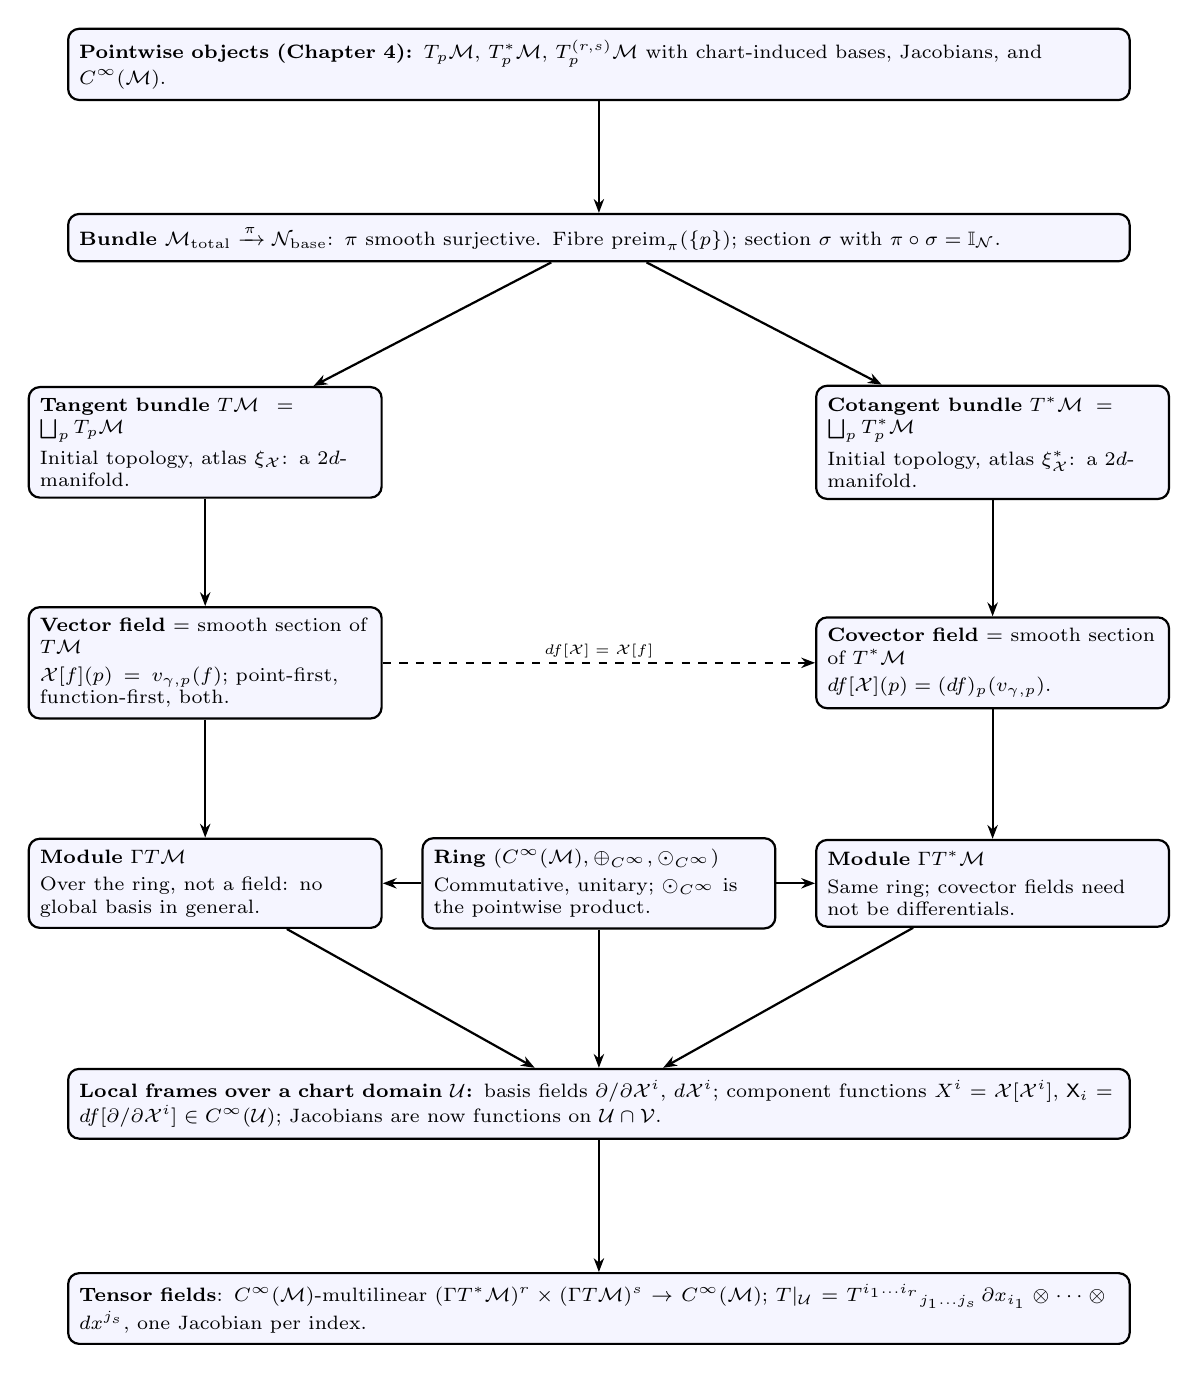
\begin{tikzpicture}[
  box/.style={draw, thick, rounded corners, fill=blue!4, align=left,
              text width=4.2cm, font=\scriptsize, inner sep=4pt},
  bigbox/.style={box, text width=13.2cm},
  aside/.style={box, fill=orange!5},
  ->, >={Stealth[length=5pt]}, thick
]

\node[bigbox] (root) at (5,0) {%
  \textbf{Pointwise objects (Chapter 4):} $T_p\mathcal M$, $T^*_p\mathcal M$, $T^{(r,s)}_p\mathcal M$
  with chart-induced bases, Jacobians, and $C^\infty(\mathcal M)$.
};

\node[bigbox] (bun) at (5,-2.2) {%
  \textbf{Bundle} $\mathcal M_{\text{total}}\xrightarrow{\pi}\mathcal N_{\text{base}}$: $\pi$ smooth surjective.
  Fibre $\mathrm{preim}_\pi(\{p\})$; section $\sigma$ with $\pi\circ\sigma=\mathbb I_{\mathcal N}$.
};

\node[box] (tm) at (0,-4.8) {%
  \textbf{Tangent bundle} $T\mathcal M=\bigsqcup_p T_p\mathcal M$\\[2pt]
  Initial topology, atlas $\xi_{\mathcal X}$: a $2d$-manifold.
};
\node[box] (tsm) at (10,-4.8) {%
  \textbf{Cotangent bundle} $T^*\mathcal M=\bigsqcup_p T^*_p\mathcal M$\\[2pt]
  Initial topology, atlas $\xi^*_{\mathcal X}$: a $2d$-manifold.
};

\node[box] (vf) at (0,-7.6) {%
  \textbf{Vector field} = smooth section of $T\mathcal M$\\[2pt]
  $\mathcal X[f](p)=v_{\gamma,p}(f)$; point-first, function-first, both.
};
\node[box] (cf) at (10,-7.6) {%
  \textbf{Covector field} = smooth section of $T^*\mathcal M$\\[2pt]
  $df[\mathcal X](p)=(df)_p(v_{\gamma,p})$.
};

\node[box] (ring) at (5,-10.4) {%
  \textbf{Ring} $(C^\infty(\mathcal M),\oplus_{C^\infty},\odot_{C^\infty})$\\[2pt]
  Commutative, unitary; $\odot_{C^\infty}$ is the pointwise product.
};
\node[box] (mod) at (0,-10.4) {%
  \textbf{Module} $\Gamma T\mathcal M$\\[2pt]
  Over the ring, not a field: no global basis in general.
};
\node[box] (smod) at (10,-10.4) {%
  \textbf{Module} $\Gamma T^*\mathcal M$\\[2pt]
  Same ring; covector fields need not be differentials.
};

\node[bigbox] (loc) at (5,-13.2) {%
  \textbf{Local frames over a chart domain $\mathcal U$:} basis fields $\partial/\partial\mathcal X^i$, $d\mathcal X^i$;
  component functions $X^i=\mathcal X[\mathcal X^i]$, $\mathsf X_i=df[\partial/\partial\mathcal X^i]\in C^\infty(\mathcal U)$;
  Jacobians are now functions on $\mathcal U\cap\mathcal V$.
};

\node[bigbox] (tf) at (5,-15.8) {%
  \textbf{Tensor fields}: $C^\infty(\mathcal M)$-multilinear $(\Gamma T^*\mathcal M)^{r}\times(\Gamma T\mathcal M)^{s}\to C^\infty(\mathcal M)$;
  $T|_{\mathcal U}=T^{i_1\dots i_r}{}_{j_1\dots j_s}\,\partial x_{i_1}\otimes\cdots\otimes dx^{j_s}$,
  one Jacobian per index.
};

\draw (root) -- (bun);
\draw (bun) -- (tm);
\draw (bun) -- (tsm);
\draw (tm) -- (vf);
\draw (tsm) -- (cf);
\draw[dashed] (vf) -- (cf) node[pos=0.5, above, font=\tiny, fill=white, inner sep=1.5pt] {$df[\mathcal X]=\mathcal X[f]$};
\draw (vf) -- (mod);
\draw (cf) -- (smod);
\draw (ring) -- (mod);
\draw (ring) -- (smod);
\draw (mod) -- (loc);
\draw (smod) -- (loc);
\draw (ring) -- (loc);
\draw (loc) -- (tf);

\end{tikzpicture}%
}
\end{center}

\end{document}
